\chapter{极小模型}
本章考虑Virasoro代数的退化表示,并介绍零模向量。所有初级场都是二重退化表示的CFT称为极小模型,是二维CFT中最基本的。极小模型中,退化初级场的关联函数满足解有固定奇点的微分方程,解它可得到共形块。此外,利用单值变换下的不变性,可以得到对关联函数的约束,算出OPE系数。我们也会解释由Dotsenko-Fateev提出的极小模型的自由场表示,这是推导关联函数的积分表示的系统方法。

\section{Virasoro代数的退化表示}
共形场论局域场的空间 $\mathcal{A} $是初级场$ \phi_i$ 所属的共形类$ [\phi_i]$ 的直和: $\mathcal{A}=\oplus_{i}\left[\phi_{i}\right]$ 。如果 $\phi_i$ 的共形权是 $(h_i,\bar{h}_i) $,共形类$ [\phi_i] $就可写成Virasoro代数右模($L_n$)和左模($\bar{L}_n$)的表示 $V_{h_{i}}, \bar{V}_{\bar{h}_{i}} $的张量积: $\left[\phi_{i}\right]=V_{h_{i}} \otimes \bar{V}_{\bar{h}_{i}} $。这里用了态-算符对应,将场和Hilbert空间中的态视作等同。Verma模 $V_h$ 由最高权态 $|h\rangle$ 和它的次级态 $L_{-n_{1}} \cdots L_{-n_{k}}|h\rangle$ ($n_{1} \geq \cdots \geq n_{k}>0$)生成。最高权态 $|h\rangle$ 满足 $L_{n}|h\rangle=0(n>0) $, $L_{0}|h\rangle=h|h\rangle $。

Verma模$ V_h $未必是Virasoro代数的不可约表示,也可能是不可约表示之和。有Verma模$V_h$的元素$|h+N\rangle$(N 是正整数)满足
\begin{align} &L_{n}|h+N\rangle=0, \quad n>0 \\ &L_{0}|h+N\rangle=(h+N)|h+N\rangle \end{align}
时,$ L_{-n} $作用在 $|h+N\rangle $上生成的空间 $V_{h+N}$ 是Virasoro代数的表示空间。这个态$ |h+N\rangle$ 称为级为 $N $的\textbf{零模向量(null vector)}或\textbf{奇异向量(singular vector)}。对应零模向量的共形场称为\textbf{零模场(null field)}。如果 $|h+N\rangle $是级为 N 的零模向量,Verma模中任何元素 $L_{-n_{1}} \cdots L_{-n_{k}}|h\rangle $与它的内积将是
\begin{equation}
	\left\langle h+N\left|L_{-n_{1}} \cdots L_{-n_{k}}\right| h\right\rangle=\left\langle h\left|L_{n_{k}} \cdots L_{n_{1}}\right| h+N\right\rangle^{*}=0
\end{equation}
特别地,它自身的范数为零: $\langle h+N | h+N\rangle=0 $。$ |h+N\rangle$ 的次级态同样与所有Verma模中元素正交。

如果Virasoro代数的表示 $V_h$ 不可约,$ V_h $就不包含零模向量。同样地,如果 $V_h$ 不包含零模向量,它就是不可约表示。$ V_h $包含一个零模向量 $|h+N\rangle$ 时, $V_h $中定义等价关系
\begin{equation}
	|h+N\rangle=0
\end{equation}
得到的空间 $[h]$ (商空间$ V_h/V_{h+N}$ )是Virasoro代数的不可约表示。这个表示 $[h]$ 称为\textbf{退化表示(degenerate representation)},$ N $称为退化表示的级。

\subsection{零模向量的组成}
Virasoro代数的最高权表示是退化表示时,可以得到共形权 $h $和中心荷$c$ 间的关系。我们构造具体的零模向量来考察这个关系。Verma模$ V_h$ 中级为 $N$ 的态可写成
$$
L_{-n_{1}} \cdots L_{-n_{k}}|h\rangle, \quad n_{1} \geq \cdots \geq n_{k}>0 \quad (N=n_{1}+\cdots+n_{k})
$$
的线性组合。

例如级为1的态形如
\begin{equation}
	|\chi\rangle=L_{-1}|h\rangle
\end{equation}
假定它是零模向量,那么作用上 $L_n$ ( $n>0 $)有
\begin{equation}
\begin{aligned} L_{n}|\chi\rangle &=L_{n} L_{-1}|h\rangle=\left(\left[L_{n}, L_{-1}\right]+L_{-1} L_{n}\right)|h\rangle \\ &=(n+1) L_{n-1}|h\rangle \\ &=0 \end{aligned}
\end{equation}
这里,我们用了Virasoro代数和$ |h\rangle $是最高权态。 $n>1$ 时,由$ |h\rangle$ 是最高权态,右边为零。$ n=1 $时,得到
$$
2 h|h\rangle=0
$$
也就是 $h=0 $。换句话说,级为1的零模向量是 $SL(2,\mathbb{C}) $不变真空 $|0\rangle $,对应的零模场是恒等算符$ \boldsymbol{I}(z) $。
级为2的态形如
\begin{equation}
|\chi\rangle=\left(L_{-2}+a L_{-1}^{2}\right)|h\rangle
\end{equation}
这里 $a$ 是常数。假定它是零模向量,用Virasoro代数,作用上$ L_n$ ( $n>0 $)有
\begin{equation}
	\begin{aligned} L_{n}|\chi\rangle=&\left(\left[L_{n}, L_{-2}\right]+a [L_{n}, L_{-1}^{2} ]\right)|h\rangle \\ =&\left\{(n+2) L_{n-2}+\frac{c}{12}\left(n^{3}-n\right) \delta_{n-2,0}+a(n+1)\left(n L_{n-2}+2 L_{-1} L_{n-1}\right)\right\}|h\rangle \\ =& 0 \end{aligned}
\end{equation}
$n=1$ 时,得到
\begin{equation}
	L_{1}|\chi\rangle=(3+2 a(2 h+1)) L_{-1}|h\rangle=0
\end{equation}
$h=0$ 时, $L_{-1}|h\rangle $是级为1的零模向量,这等式成立。 $h\neq 0 $时,得到
\begin{equation}
	a=-\frac{3}{2(2 h+1)}
\end{equation}
$n=2 $时,得到
\begin{equation}
L_{2}|\chi\rangle=\left(4 h+\frac{c}{2}+6 a h\right)|h\rangle=0
\end{equation}
于是有关于 $h,c $的方程
\begin{equation}
	(6 a+4) h+\frac{c}{2}=0
\end{equation}
代入 (5.10) 得到 $h,c$ 间的关系
\begin{equation}
	8 h^{2}+(c-5) h+\frac{c}{2}=0
\end{equation}
$n\geq 3$ 时不会得到新等式。总结一下,$ h,c $满足 (5.13) 时,
\begin{equation}
	\left(L_{-2}-\frac{3}{2(2 h+1)} L_{-1}^{2}\right)|h\rangle
\end{equation}
是级为2的零模向量。 (5.13) 是关于 $h$ 的二次方程,对给定中心荷 $c$ ,$ h $有两取值
\begin{equation}
	h=\frac{5-c \pm \sqrt{c^{2}-26 c+25}}{16}
\end{equation}
级为3的态形如
\begin{equation}
	|\chi\rangle=\left(L_{-3}+a L_{-2} L_{-1}+b L_{-1}^{3}\right)|h\rangle
\end{equation}
这里 $a,b $是常数。假定它是零模向量,作用上Virasoro算符$ L_n $( $n>0$ )有
\begin{equation}
	\begin{aligned} L_{n}|\chi\rangle=&\Big\{(n+3) L_{n-3}+\frac{c}{12}\left(n^{3}-n\right) \delta_{n-3,0} \\ &+a \big[(n+2)(n-1) L_{n-3}+(n+1) L_{-2} L_{n-1} \\ &\quad +(n+2) L_{-1} L_{n-2}+\frac{c}{12} (n^{3}-n ) \delta_{n-2,0} L_{-1} \big] \\ &+b(n+1) (3 n L_{-1} L_{n-2}+n(n-1) L_{n-3} +3 L_{-1}^{2} L_{n-1} ) \Big\}|h\rangle \\=&0 \end{aligned}
\end{equation}
$n=1 $时,得到
\begin{equation}
	L_{1}|\chi\rangle=\left\{(4+2 a h) L_{-2}+(3 a+3 b(2 h+2)) L_{-1}^{2}\right\}|h\rangle=0
\end{equation}
于是
\begin{equation}
	4+2 a h=0, \quad 3 a+6 b(h+1)=0
\end{equation}
$n=2 $时,得到
\begin{equation}
	5+a\left(4+4 h+\frac{c}{2}\right)+3 b(6 h+2)=0
\end{equation}
$n=3$ 时,得到
\begin{equation}
	6 h+2 c+10 a h+24 b h=0
\end{equation}
这最后一个等式是多余的,只需要前三个等式。可以得到级为3的零模向量是
\begin{equation}
\left(L_{-3}-\frac{2}{h} L_{-2} L_{-1}+\frac{1}{h( h+1)} L_{-1}^{3}\right)|h\rangle
\end{equation}
其中
\begin{equation}
	h=\frac{7-c \pm \sqrt{c^{2}-26 c+25}}{6}
\end{equation}
从级为2和3的例子中可以看到,零模向量对应的共形权有特别的形式。引入参数
\begin{equation}
\alpha_{\pm}=\frac{\sqrt{1-c} \pm \sqrt{25-c}}{\sqrt{24}}
\end{equation}
$\alpha_{\pm} $满足
\begin{align} &\alpha_{+} \alpha_{-}=-1 \\ &\left(\alpha_{+}+\alpha_{-}\right)^{2}=\frac{1-c}{6}, \quad\left(\alpha_{+}-\alpha_{-}\right)^{2}=\frac{25-c}{6}  \end{align}
中心荷$ c $可用 $\alpha_{\pm} $写成
\begin{equation}
	c=1-6\left(\alpha_{+}+\alpha_{-}\right)^{2}
\end{equation}
再引入
\begin{equation}
	h_{0}=-\frac{1}{4}\left(\alpha_{+}+\alpha_{-}\right)^{2}=\frac{c-1}{24}
\end{equation}
对正整数 $n,m $定义
\begin{equation}
	h_{n, m}=h_{0}+\frac{1}{4}\left(n \alpha_{+}+m \alpha_{-}\right)^{2}
\end{equation}
$h_{n,m} $写成 $c$ 的函数是
\begin{equation}
	\begin{aligned} h_{n, m}=&\frac{1}{4}\left(n^{2}-1\right) \alpha_{+}^{2}+\frac{1}{4}\left(m^{2}-1\right) \alpha_{-}^{2}-\frac{1}{2}(m n-1) \\ =& \frac{1}{48}\Big\{-24(m n-1)+\left(n^{2}+m^{2}-2\right)(13-c)\\&+\left(n^{2}-m^{2}\right) \sqrt{(1-c)(25-c)}\Big\} \end{aligned}
\end{equation}
$n,m $较小时的几个值是
\begin{equation*}
	\begin{aligned} &h_{1,1}=0 \\& h_{1,2}=\frac{5-c-\sqrt{(1-c)(25-c)}}{16} \quad h_{2,1}=\frac{5-c+\sqrt{(1-c)(25-c)}}{16} \\& h_{1,3}=\frac{7-c-\sqrt{(1-c)(25-c)}}{6} \quad h_{3,1}=\frac{7-c+\sqrt{(1-c)(25-c)}}{6} \end{aligned}
\end{equation*}
这些共形权对应级为1, 2, 3的零模向量。

一般来说,对正整数$ n,m $,共形权$ h=h_{n,m}$ 对应级为$ N=nm $的零模向量。 (5.29) 也称为Kac谱。最高权态$ \left|h_{n, m}\right\rangle \otimes\left|h_{n, m}\right\rangle $对应的初级场记作 $\phi_{(n, m)}(z, \bar{z}) $。文献\footnote{L. Benoit and Y. Saint-Aubin, Phys. Lett. B 215 (1988) 517.}\footnote{M. Bauer, P. Di Francesco, C. Itzykson and J. B. Zuber, Nucl. Phys. B 362 (1991) 515.}中讨论了如何构造Virasoro代数的零模向量。

\section{零模场的关联函数}
考虑包含初级场 $\phi_{(n, m)}(z, \bar{z}) $的关联函数,它的共形类中有Kac谱中的零模场:
$$
\left\langle\phi_{(n, m)}(z) \phi_{1}\left(z_{1}\right) \cdots \phi_{N}\left(z_{N}\right)\right\rangle
$$
这里忽略了对 $\bar{z} $的依赖。

因为可由$ \phi_{(n, m)}(z) $得到的零模场 $\chi_{(n, m)}(z)$ 在关联函数中会给出零,可以推出关联函数需要满足的新微分方程。\footnote{由态-算符对应,两算符的关联函数正比于对应态的内积,多个算符的可通过OPE转化成两个的,而零模向量与其它态都正交,那么关联函数为零。}级为1的零模场$ \chi_{(1,1)}(z)$ 是恒等算符 $\boldsymbol{I}(z)$ ,不依赖于坐标 $z $:由 (4.17),(4.28) ,这零模场满足 $\left(L_{-1} \boldsymbol{I}\right)(z)=\partial_{z} \boldsymbol{I}(z)=0$。在关联函数中,这给出
$$
\left\langle\left(L_{-1} \boldsymbol{I}\right)(z) \phi_{1}\left(z_{1}\right) \cdots \phi_{N}\left(z_{N}\right)\right\rangle=\partial_{z}\left\langle\boldsymbol{I}(z) \phi_{1}\left(z_{1}\right) \cdots \phi_{N}\left(z_{N}\right)\right\rangle=0
$$
这等式就是在表达关联函数不依赖于 $z$ ,是平凡的。

初级场 $\phi_{(1,2)}(z) $的共形类中有级为2的零模场
\begin{equation}
	\chi_{(1,2)}(z)=\left(\left(L_{-2}-\frac{3}{2\left(2 h_{1,2}+1\right)} L_{-1}^{2}\right) \phi_{(1,2)}\right)(z)
\end{equation}
关联函数 $\left\langle\chi_{(1,2)}(z) \phi_{1}\left(z_{1}\right) \cdots \phi_{N}\left(z_{N}\right)\right\rangle $为零,由 (5.31),(4.35) 有
\begin{equation}
\begin{aligned} &\left\langle\left(\left(L_{-2}-\frac{3}{2\left(2 h_{1,2}+1\right)} L_{-1}^{2}\right) \phi_{(1,2)}\right)(z) \phi_{1}\left(z_{1}\right) \cdots \phi_{N}\left(z_{N}\right)\right\rangle \\ =&\left(\mathcal{L}_{-2}-\frac{3}{2\left(2 h_{1,2}+1\right)} \mathcal{L}_{-1}^{2}\right)\left\langle\phi_{(1,2)}(z) \phi_{1}\left(z_{1}\right) \cdots \phi_{N}\left(z_{N}\right)\right\rangle \\ =& 0 \end{aligned}
\end{equation}
代入 $\mathcal{L}_{-1}=\partial_{z}$ 以及 (4.36) 给出的 $\mathcal{L}_{-2}$ ,得到微分方程
\begin{equation}
	\begin{aligned} &\left\{\frac{3}{2\left(2 h_{1,2}+1\right)} \frac{\partial^{2}}{\partial z^{2}}-\sum_{i=1}^{N}\left[\frac{h_{i}}{\left(z-z_{i}\right)^{2}}+\frac{1}{z-z_{i}} \frac{\partial}{\partial z_{i}}\right]\right\} \\& \times\left\langle\phi_{(1,2)}(z) \phi_{1}\left(z_{1}\right) \cdots \phi_{N}\left(z_{N}\right)\right\rangle=0 \end{aligned}
\end{equation}
同样地,对共形类中有级为3的零模场的初级场$ \phi_{(1,3)}(z) $,有三阶微分方程
\begin{equation}
	\begin{aligned} &\left\{\frac{1}{ h_{1,3}+1} \frac{\partial^{3}}{\partial z^{3}}-\sum_{i=1}^{N}\left[\frac{2 h_{1,3} h_{i}}{\left(z-z_{i}\right)^{3}}+\frac{h_{1,3}}{\left(z-z_{i}\right)^{2}} \frac{\partial}{\partial z_{i}}+\frac{2 h_{i}}{\left(z-z_{i}\right)^{2}} \frac{\partial}{\partial z}+\frac{2}{z-z_{i}} \frac{\partial^{2}}{\partial z_{i} \partial z}\right]\right\} \\&\quad \times\left\langle\phi_{(1,3)}(z) \phi_{1}\left(z_{1}\right) \cdots \phi_{N}\left(z_{N}\right)\right\rangle=0 \end{aligned}
\end{equation}

一般来说,共形类中有级为$ N=nm$ 的零模场的退化初级场 $\phi_{(n, m)} $满足一个 $nm $阶微分方程。这些微分方程是Virasoro代数退化表示给出的关联函数的新约束。

\subsection{四点函数}
例如,考虑四点函数 $\left\langle\phi_{(1,2)}(z) \phi_{1}\left(z_{1}\right) \phi_{2}\left(z_{2}\right) \phi_{3}\left(z_{3}\right)\right\rangle$ 满足的微分方程。定义 $\phi_{0}\left(z_{0}\right)=\phi_{(1,2)}(z) $, $h_{0}=h_{1,2}$ ,引入交比
$$
x=\frac{z_{01} z_{23}}{z_{02} z_{13}}, \quad z_{i j}=z_{i}-z_{j}
$$
(4.64) 变成了
\begin{equation}
\begin{aligned} &\left\langle\phi_{0}\left(z_{0}\right) \phi_{1}\left(z_{1}\right) \phi_{2}\left(z_{2}\right) \phi_{3}\left(z_{3}\right)\right\rangle \\ =&\left(\frac{z_{13}}{z_{10} z_{03}}\right)^{h_{0}}\left(\frac{z_{30}}{z_{13} z_{10}}\right)^{h_{1}}\left(\frac{z_{10} z_{30}}{z_{13} z_{20}^{2}}\right)^{h_{2}}\left(\frac{z_{10}}{z_{13} z_{30}}\right)^{h_{3}} G_{32}^{10}(x) \end{aligned}
\end{equation}
其中
\begin{equation}
	G_{32}^{10}(x)=x^{a_{1}}(1-x)^{b_{1}} H(x) 
\end{equation}
$a_{1}=h_{0}+h_{1}-h_{2}-h_{3}$ ,$ b_{1}=h_{0}-h_{1}-h_{2}+h_{3}$ , $H(x)$ 满足微分方程
\begin{equation}
\begin{aligned} &\frac{3}{2\left(1+2 h_{0}\right)} \frac{d^{2} H(x)}{d x^{2}}+\frac{1-2 x}{x(1-x)} \frac{d H(x)}{d x} \\& -\left\{\frac{\lambda}{x(1-x)}+\frac{h_{1}}{x^{2}}+\frac{h_{3}}{(1-x)^{2}}\right\} H(x)=0 \end{aligned}
\end{equation}
其中 $\lambda=h_{0}+h_{1}-h_{2}+h_{3}$ 。\footnote{计算的中间结果可见P. Di Francesco et al., Conformal Field Theory, pp. 252-254.}

微分方程 (5.37) 是一个解有固定奇点 $x=0,1,\infty$ 的Fuchs型微分方程。记
\begin{equation}
	H(x)=x^{a_{2}}(1-x)^{b_{2}} F(x), \quad \frac{3}{2\left(1+2 h_{0}\right)}=\frac{1}{t}
\end{equation}
(5.30) 给出
$$
h_{1,2}=\frac{3}{4} \alpha_{-}^{2}-\frac{1}{2}
$$
于是
$$
\frac{3}{2\left(1+2 h_{0}\right)}=\frac{1}{\alpha_{-}^{2}}
$$
也就是$ t=\alpha_-^2 $。微分方程 (5.37) 可重写成
\begin{equation}
	\begin{aligned} &x(1-x) \frac{d^{2} F}{d x^{2}}+\left(t+2 a_{2}-2\left(t+a_{2}+b_{2}\right) x\right) \frac{d F}{d x} \\& +\Bigg\{-\left(a_{2}+b_{2}+t-\frac{1}{2}\right)^{2}+\left(t-\frac{1}{2}\right)^{2}-\left(h_{0}-h_{2}\right) t\\&\quad +\frac{a_{2}\left(a_{2}-1\right)+t a_{2}-h_{1} t}{x}+\frac{b_{2}\left(b_{2}-1\right)+t b_{2}-h_{2} t}{1-x}\Bigg\} F=0 \end{aligned}
\end{equation}
我们选取 $a_2,b_2 $以使$ 1/x,1/(1-x)$ 的系数为零,那么
\begin{equation}
	a_{2}=\frac{1-t \pm \sqrt{(t-1)^{2}+4 h_{1} t}}{2}, \quad b_{2}=\frac{1-t \pm \sqrt{(t-1)^{2}+4 h_{3} t}}{2}
\end{equation}
可以看到 $F(x)$ 满足超几何微分方程
\begin{equation}
	x(1-x) \frac{d^{2} F}{d x^{2}}+(\gamma-(\alpha+\beta+1) x) \frac{d F}{d x}-\alpha \beta F=0
\end{equation}
其中
\begin{equation}
	\begin{aligned} &\alpha=a_{2}+b_{2}+t-\frac{1}{2}+\sqrt{\left(t-\frac{1}{2}\right)^{2}-\left(h_{0}-h_{2}\right) t} \\& \beta=a_{2}+b_{2}+t-\frac{1}{2}-\sqrt{\left(t-\frac{1}{2}\right)^{2}-\left(h_{0}-h_{2}\right) t} \\& \gamma=t+2 a_{2} \end{aligned}
\end{equation}
不过, $\alpha,\beta$ 可以互换。定义参数$ \alpha$ 的函数\footnote{与 (5.41) 中的 $\alpha $无关}
\begin{equation}
	h(\alpha)=\frac{1}{4} \alpha^{2}-\frac{1}{4}\left(\alpha_{+}+\alpha_{-}\right)^{2}
\end{equation}
可将初级场 $\phi_1,\phi_2,\phi_3 $的共形权$ h_1,h_2,h_3 $写成 $h_{i}=h\left(\alpha_{i}\right) $。 $h_{0}=h_{1,2}=h\left(\alpha_{+}+2 \alpha_{-}\right) $。于是$ a_2,b_2$ 可写成
$$
a_{2}=\frac{1-t \pm \alpha_{1} \sqrt{t}}{2}, \quad b_{2}=\frac{1-t \pm \alpha_{3} \sqrt{t}}{2}
$$
简单起见取负号,我们得到
\begin{equation}
	\begin{aligned} &\alpha=\frac{1}{2}\left(1-\sqrt{t}\left(\alpha_{1}+\alpha_{2}+\alpha_{3}\right)\right) \\& \beta=\frac{1}{2}\left(1-\sqrt{t}\left(\alpha_{1}-\alpha_{2}+\alpha_{3}\right)\right) \\& \gamma=1-\alpha_{1} \sqrt{t} \end{aligned}
\end{equation}
以及
\begin{equation}
	a_{2}=h\left(\alpha_{1}-\alpha_{-}\right)-h_{1,2}-h\left(\alpha_{1}\right), \quad b_{2}=h\left(\alpha_{3}-\alpha_{-}\right)-h_{1,2}-h\left(\alpha_{3}\right)
\end{equation}
考虑超几何微分方程 (5.41) 在$ x=0 $附近的级数解
$$
F=x^{\lambda}\left(1+\sum_{n=1}^{\infty} a_{n} x^{n}\right)
$$
指数$ \lambda $满足方程
$$
\lambda^{2}+(\gamma-1) \lambda=0
$$
解得 $\lambda=0,1-\gamma $。 $\lambda=0 $的解记作$ F_1 $,称为超几何级数,定义为
\begin{equation}
	F_{1}(x)=F(\alpha, \beta, \gamma, x)=\sum_{n=0}^{\infty} \frac{(\alpha)_{n}(\beta)_{n}}{(1)_{n}(\gamma)_{n}} x^{n}
\end{equation}
其中
\begin{equation}
	\begin{array}{l} (x)_{n}=x(x+1) \cdots(x+n-1) \quad(n=1,2, \cdots)\\ (x)_{0}=1 \end{array}
\end{equation}
特别地, $(1)_{n}=n ! $。 $\lambda=1-\gamma $的解记作$ F_2 $,可用超几何级数写成
\begin{equation}
	F_{2}(x)=x^{1-\gamma} F(\alpha-\gamma+1, \beta-\gamma+1,2-\gamma, x)
\end{equation}
任何解都可写成线性组合$ F=c_{1} F_{1}+c_{2} F_{2} $。

那么关联函数$ G_{32}^{10}(x) $可用超几何级数写成
\begin{equation}
	\begin{aligned} G_{32}^{10}(x)=& c_{1} x^{a_{1}+a_{2}}(1-x)^{b_{1}+b_{2}} F(\alpha, \beta, \gamma, x) \\ &+c_{2} x^{a_{1}+a_{2}+1-\gamma}(1-x)^{b_{1}+b_{2}} F(\alpha-\gamma+1, \beta-\gamma+1,2-\gamma, x) \end{aligned}
\end{equation}
由 $a_1,b_1 $的定义以及 (5.44),(5.45) ,我们有
\begin{align} &a_{1}+a_{2}=h\left(\alpha_{1}-\alpha_{-}\right)-h_{2}-h_{3} \\& b_{1}+b_{2}=h\left(\alpha_{3}-\alpha_{-}\right)-h_{1}-h_{2}\\& a_{1}+a_{2}+1-\gamma=h\left(\alpha_{1}+\alpha_{-}\right)-h_{2}-h_{3} \end{align}
系数 $c_1,c_2$ 可由关联函数在单值变换下的不变性确定,这将在5.6节解释。各项都代表共形块。我们可从 $x$ 的幂次直接看出$ h_p $的值: (5.49) 的第一项对应 $h_{p}=h\left(\alpha_{1}-\alpha_{-}\right)$ ,第二项对应 $h_{p}=h\left(\alpha_{1}+\alpha_{-}\right)$ 。这表征了初级场 $\phi_{(1,2)}$ 和 $\phi_1 $的OPE的代数结构。这OPE的代数结构将在下节解释。

\section{融合规则}

我们来详细考察退化初级场OPE代数的结构,这是从零模场的微分方程推出的。在关联函数$ \left\langle\phi_{(1,2)}(z) \phi_{1}\left(z_{1}\right) \cdots \phi_{N}\left(z_{N}\right)\right\rangle $中,设退化初级场 $\phi_{(1,2)}(z)$ 和共形权是 $h_1 $的初级场 $\phi_1(z_1)$ 的OPE是
\begin{equation}
	\phi_{(1,2)}(z) \phi_{1}\left(z_{1}\right)=\sum_{k} C_{(1,2) 1}^{k}\left(z-z_{1}\right)^{h_{k}-h_{1}-h_{1,2}}\left[\phi_{k}\left(z_{1}\right)+\cdots\right]
\end{equation}
将这OPE代入关联函数的微分方程 (5.33) 。极限 $z\to z_1 $下最奇异的项是
\begin{equation}
\sum_{k} C_{(1,2) 1}^{k}\left\{\frac{3}{2\left(2 h_{1,2}+1\right)} \kappa_{k}\left(\kappa_{k}-1\right)-h_{1}+\kappa_{k}\right\}\left(z-z_{1}\right)^{\kappa_{k}-2}\left\langle\phi_{k}\left(z_{1}\right) \cdots\right\rangle	
\end{equation}
其中 $\kappa_{k}=h_{k}-h_{1}-h_{1,2} $。因此 $\kappa_k$ 满足
\begin{equation}
	\frac{3}{2\left(2 h_{1,2}+1\right)} \kappa_{k}\left(\kappa_{k}-1\right)-h_{1}+\kappa_{k}=0
\end{equation}
由这方程解得
\begin{equation}
h_{k}=\frac{1}{6}\left(1+6 h_{1}+2 h_{1,2} \pm \sqrt{1+24 h_{1}-8 h_{1,2}+48 h_{1} h_{1,2}+16 h_{1,2}^{2}}\right)	
\end{equation}
零模场的微分方程确定了 $h_k $的值。这个解形式复杂,但如果记$ h_1=h(\alpha)$ ,$ h_k $就可写成
\begin{equation}
	h\left(\alpha-\alpha_{-}\right), \quad h\left(\alpha+\alpha_{-}\right)
\end{equation}
共形权是$ h=h(\alpha)$ 的初级场记作$ \phi_{(\alpha)}$ 。我们只考虑OPE的结果中初级场所属的共形类,那么 $\phi_{(1,2)}$ 和 $\phi_{(\alpha)}$ 的OPE表达了如下的初级场共形类间的关系:
\begin{equation}
	\left[\phi_{(1,2)}\right]\left[\phi_{(\alpha)}\right]=\left[\phi_{\left(\alpha-\alpha_{-}\right)}\right]+\left[\phi_{\left(\alpha+\alpha_{-}\right)}\right]
\end{equation}
这称为\textbf{融合规则(fusion rule)}。$ \phi_{(2,1)} $对应的融合规则是
\begin{equation}
	\left[\phi_{(2,1)}\right]\left[\phi_{(\alpha)}\right]=\left[\phi_{\left(\alpha-\alpha_{+}\right)}\right]+\left[\phi_{\left(\alpha+\alpha_{+}\right)}\right]
\end{equation}
$\phi_{(1,2)} $同时也是 $\phi_{\left(\alpha_{+}+2 \alpha_{-}\right)} $,那么特别地, $\phi_{(1,2)}$ 和 $\phi_{(1,2)} $的融合规则是
\begin{equation}
	\left[\phi_{(1,2)}\right]\left[\phi_{(1,2)}\right]=\left[\phi_{(1,1)}\right]+\left[\phi_{(1,3)}\right]
\end{equation}

考虑融合规则的代数性质时,也称它为\textbf{融合代数(fusion algebra)}。OPE代数有结合律,那么融合规则就有结合律,自然地也有分配律。 (5.60) 两边作用在 $[\phi(\alpha)] $上。由(5.58),左边是
\begin{equation}
	\begin{aligned} \left(\left[\phi_{(1,2)}\right]\left[\phi_{(1,2)}\right]\right)\left[\phi_{(\alpha)}\right] &=\left[\phi_{(1,2)}\right]\left(\left[\phi_{(1,2)}\right]\left[\phi_{(\alpha)}\right]\right) \\ &=\left[\phi_{(1,2)}\right]\left(\left[\phi_{\left(\alpha-\alpha_{-}\right)}\right]+\left[\phi_{\alpha+\alpha_{+}}\right]\right) \\ &=\left[\phi_{\left(\alpha-2 \alpha_{-}\right)}\right]+2\left[\phi_{(\alpha)}\right]+\left[\phi_{\left(\alpha+2 \alpha_{-}\right)}\right] \end{aligned}
\end{equation}
另一方面,$ \phi_{(1,1)} $是恒等算符,那么 (5.60) 的右边是
\begin{equation}
	\left[\phi_{(\alpha)}\right]+\left[\phi_{(1,3)}\right]\left[\phi_{(\alpha)}\right]
\end{equation}
这意味着
\begin{equation}
	\left[\phi_{(1,3)}\right]\left[\phi_{(\alpha)}\right]=\left[\phi_{\left(\alpha-2 \alpha_{-}\right)}\right]+\left[\phi_{(\alpha)}\right]+\left[\phi_{\left(\alpha+2 \alpha_{-}\right)}\right]
\end{equation}
重复这样的操作,可以得到 $\phi_{(1, m)} $和 $\phi_{(\alpha)}$ 的融合规则是
\begin{equation}
	\begin{aligned} \left[\phi_{(1, m)}\right]\left[\phi_{(\alpha)}\right] &=\left[\phi_{\left(\alpha+(-m+1) \alpha_{-}\right)}\right]+\left[\phi_{\left(\alpha+(-m+3) \alpha_{-}\right)}\right]+\cdots+\left[\phi_{\left(\alpha+(m-1) \alpha_{-}\right)}\right] \\ &=\sum_{l=0}^{m-1}\left[\phi_{\left(\alpha+(2 l-m+1) \alpha_{-}\right.}\right] \end{aligned}
\end{equation}
对这进行推广,一般的退化初级场 $\phi_{(n, m)}$ 和初级场$ \phi_{(\alpha)} $的融合规则是
\begin{equation}
	\left[\phi_{(n, m)}\right]\left[\phi_{(\alpha)}\right]=\sum_{k=0}^{n-1} \sum_{l=0}^{m-1}\left[\phi_{\left(\alpha+(2 k-n+1) \alpha_{+}+(2 l-m+1) \alpha_{-}\right)}\right]
\end{equation}
我们这里应当注意退化初级场间的融合规则。例如 $\phi_{(1,2)} $和 $\phi_{(2,1)}$ 的, $\phi_{(2,1)} $和 $\phi_{(1,2)}$ 的,似乎应当是
\begin{equation}
\begin{array}{l} {\left[\phi_{(1,2)}\right]\left[\phi_{(2,1)}\right] \stackrel{?}{=}\left[\phi_{(2,0)}\right]+\left[\phi_{(2,2)}\right]} \\ {\left[\phi_{(2,1)}\right]\left[\phi_{(1,2)}\right] \stackrel{?}{=}\left[\phi_{(0,2)}\right]+\left[\phi_{(2,2)}\right]} \end{array}
\end{equation}
两个融合规则应当一样,可是这里一个是 $\left[\phi_{(2,0)}\right]$ ,一个是 $\left[\phi_{(0,2)}\right] $。其实,OPE系数$ C_{(1,2)(2,1)}^{(2,0)}$ 和 $C_{(2,1)(1,2)}^{(0,2)} $为零,这里默认不是了。如果系数为零,融合代数将是
\begin{equation}
	\begin{array}{l} {\left[\phi_{(1,2)}\right]\left[\phi_{(2,1)}\right]=\left[\phi_{(2,2)}\right]} \\ {\left[\phi_{(2,1)}\right]\left[\phi_{(1,2)}\right]=\left[\phi_{(2,2)}\right]} \end{array}
\end{equation}

这样融合规则的定义是一致的。OPE系数的具体计算之后再说,这里只给出结果:不属于Kac谱,也就是共形权不是 $h_{n,m} $( $n,m $是正整数),而是例如 $h_{0,m}$ , $h_{n,0} $等的场,不会出现在融合规则的右边。那么,退化初级场 $\phi_{\left(n_{1}, m_{1}\right)}$ , $\phi_{\left(n_{2}, m_{2}\right)} $的融合规则关于Kac谱中的初级场是封闭的。例如,考虑 $\phi_{\left(1, m_{1}\right)}$ 和 $\phi_{\left(1, m_{2}\right)} $的,在 (5.64) 中令 $\alpha=\alpha_{+}+m_{2} \alpha_{-}$ 得到
\begin{equation}
	\begin{aligned} \left[\phi_{\left(1, m_{1}\right)}\right]\left[\phi_{\left(1, m_{2}\right)}\right] &=\left[\phi_{\left(1, m_{2}-m_{1}+1\right)}\right]+\cdots+\left[\phi_{\left(1, m_{2}+m_{1}-1\right)}\right] \\ & \stackrel{?}{=} \sum_{k=0}^{m_{1}-1}\left[\phi_{\left(1, m_{2}-m_{1}+2 k+1\right)}\right] \end{aligned}
\end{equation}
但融合规则的右边不会出现 $m_{2}-m_{1}+2 k+1<0 $的项。我们来考虑$ k $要满足的条件。如果 $m_{2}-m_{1} \geq 0 $,那么 $k=0, \cdots, m_{1}-1 $都行。如果 $m_{2}-m_{1}<0 $,考虑 $\phi_{\left(1, m_{1}\right)} $和 $\phi_{\left(1, m_{2}\right)} $互换后的融合规则
\begin{equation}
	\left[\phi_{\left(1, m_{2}\right)}\right]\left[\phi_{\left(1, m_{1}\right)}\right] \stackrel{?}{=} \sum_{k=0}^{m_{2}-1}\left[\phi_{\left(1, m_{1}-m_{2}+2 k+1\right)}\right]
\end{equation}
右边的场在 $k=0, \cdots, m_{2}-1$ 时都属于Kac谱。这可统一写成
\begin{equation}
	\left[\phi_{\left(1, m_{1}\right)}\right]\left[\phi_{\left(1, m_{2}\right)}\right]=\sum_{k=0}^{\min \left(m_{1}, m_{2}\right)-1}\left[\phi_{\left(1,\left|m_{1}-m_{2}\right|+2 k+1\right)}\right]
\end{equation}
$\min \left(m_{1}, m_{2}\right) $指 $m_1,m_2 $中更小的数。于是一般的退化初级场间融合规则是
\begin{equation}
	\left[\phi_{\left(n_{1}, m_{1}\right)}\right]\left[\phi_{\left(n_{2}, m_{2}\right)}\right]=\sum_{k=0}^{\min \left(n_{1}, n_{2}\right)-1 } \sum_{l=0}^{\min \left(m_{1}, m_{2}\right)-1}\left[\phi_{\left(\left|n_{1}-n_{2}\right|+2 k+1,\left|m_{1}-m_{2}\right|+2 l+1\right)}\right]
\end{equation}
这也可写成
\begin{equation}
	\left[\phi_{\left(n_{1}, m_{1}\right)}\right]\left[\phi_{\left(n_{2}, m_{2}\right)}\right]=\sum_{k=\left|n_{1}-n_{2}\right|+1}^{n_{1}+n_{2}-1} \sum_{l=\left|m_{1}-m_{2}\right|+1}^{m_{1}+m_{2}-1}\left[\phi_{(k, l)}\right]
\end{equation}
注意当$n_1+n_2$为奇数时,$k$对偶数求和,反之对奇数求和,对$l$求和同理。在初级场的OPE代数中,退化初级场的OPE是封闭的。

\section{极小模型}
在Belavin-Polyakov-Zamolodchikov的论文\footnote{A. A. Belavin, A. M. Polyakov and A. B. Zamolodchikov, Nucl. Phys. B 241 (1984) 333.}中,考虑了所有初级场都属于退化表示的共形场论。为使共形场论在物理上有意义,考虑的是Hilbert空间上内积正定,共形权非复也非负\footnote{非酉CFT中则是容许的。}的。

\begin{figure}[h]
	\centering
	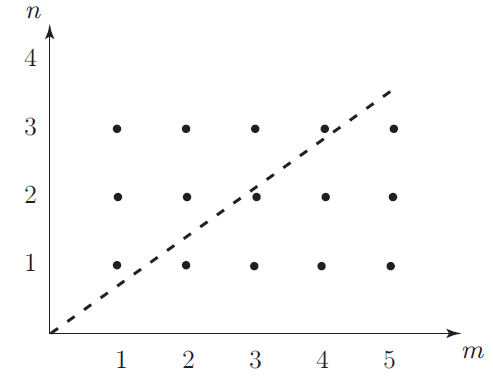
\includegraphics[width=0.6\linewidth]{fig/5.1.png}
	\caption{Kac谱的格点图。}
\end{figure}

我们来考察什么样的共形场论符合这要求。由 (5.24) ,中心荷 $c $满足$ 1<c<25$ 时,$ \alpha_\pm$ 是复的,Kac谱中的共形权 $h_{n,m}$ 一般也是复的。因此,退化初级场给出的中心荷 $c$ 有限制 $c\leq 1 $或$c\geq 25$ 。$ c\geq 25$时, $\alpha_\pm$ 是纯虚数,如果$n,m $足够大,共形权 $h_{n,m}$ 将是负的。因此考虑 $c\leq 1$ 。退化初级场的共形权由二维中坐标为$ (m,n) $的格点代表,如图5.1。虚线是斜率为
$$
\tan \theta=-\frac{\alpha_{-}}{\alpha_{+}}
$$
的直线。对一般的 $c<1 $, $\alpha_-/\alpha_+ $是无理数,虚线上没有格点。但可以看到, $(m,n)$ 取值合适时,格点可以任意接近虚线。这时,$ \left(n \alpha_{+}+m \alpha_{-}\right)^{2} $\footnote{由解析几何不难知道,这个量与点$ (n,m) $到直线$ n=-\alpha_- m/\alpha_+ $的距离正相关}可以任意小,因此存在使得 $h_{n,m}<0$ 的格点。

如果斜率是有理数呢?
\begin{equation}
\tan \theta=-\frac{\alpha_{-}}{\alpha_{+}}=\frac{q}{p}, \quad p, q \in \mathbb{Z}, \quad p>q
\end{equation}
这时, $p \alpha_{-}+q \alpha_{+}=0$ ,初级场间有了新的关系。由 (5.29) ,初级场 $\phi_{(n, m)}$ 的共形权 $h_{n,m} $满足
\begin{align} &h_{n+q, m+p}=h_{n, m}\\ &h_{q-n, p-m}=h_{n, m} \\ &h_{n, m}+n m=h_{n+q, p-m}=h_{q-n, p+m} \\ &h_{n, m}+(q-n)(p-m)=h_{n, 2 p-m}=h_{2 q-n, m} \end{align}
这说明,初级场 $\phi_{(n, m)} $的Verma模中级为$ nm$($(q-n)(p-m)$)的零模态,属于初级场 $\phi_{(n+q, p-m)}$ 或 $\phi_{(q-n, p+m)}$( $\phi_{(n, 2p-m)}$ 或 $\phi_{(2q-n, m)}$)的Kac谱。因此, $\alpha_-/\alpha_+$ 是有理数时,初级场 $\phi_{(n, m)}$ 有级为 $nm$ 和 $(q-n)(p-m)$ 的零模场。\footnote{[这句话初看起来似乎有点绕口,其实就是在说$\phi_{(n,m)}$的$nm$级次级态的共形权刚好是$\phi_{(n+q,p-m)}$(或者$\phi_{(q-n,p+m)}$)的共形权,极小模型认为共形权不存在简并,所以这个初级场就是个零模,那么这个初级场就要被剔除掉。]}

令零模场等价成$0$,可以得到Virasoro代数的不可约表示。可以看到,Kac谱中只剩下有限个独立的初级场,对应$ n=1,2,...,q-1$ , $m=1,2,...,p-1$ 。此外,根据对称性 (5.75) 令 $\phi_{(q-n, p-m)} $和 $\phi_{(n, m)}$ 等价,就只剩下 $(p-1)(q-1)/2 $个初级场。接着,由$ p \alpha_{-}+q \alpha_{+}=0 $和 $\alpha_{+} \alpha_{-}=-1 $解得
\begin{equation}
	\alpha_{-}=\sqrt{\frac{q}{p}}, \quad \alpha_{+}=-\sqrt{\frac{p}{q}}
\end{equation}
那么中心荷和共形权就是
\begin{align} &c=1-6\left(\alpha_{+}+\alpha_{-}\right)^{2}=1-6 \frac{(p-q)^{2}}{p q} \\ &h_{n, m}=\frac{(n p-m q)^{2}-(p-q)^{2}}{4 p q} \end{align}
一般来说,这样的共形场论中初级场是有限个,而不是通常的无穷个,称为\textbf{极小模型}。

我们来考察$ 0<n<q$ , $0<m<p$ 的格点上的初级场融合代数的具体结构。 $(p,q)=(3,2) $时,有$ \phi_{(1,1)} $和$ \phi_{(1,2)}$ ,但对称性 (5.75) 给出 $\phi_{(1,1)}=\phi_{(1,2)} $。因此这个理论中只有恒等算符 $\boldsymbol{I}=\phi_{(1,1)} $,中心荷是 $c=0$ 。非平凡的理论例如 $(p,q)=(5,2)$ 或 $(p,q)=(4,3)$ ,接下来考察一个例子。

$(p,q)=(5,2) $模型的Kac谱中,有初级场 $\phi_{(1,1)} $, $\phi_{(1,2)}$ , $\phi_{(1,3)} 和 \phi_{(1,4)}$ 。对称性给出$ \phi_{(1,3)}=\phi_{(1,2)}$ , $\phi_{(1,4)}=\phi_{(1,1)}$ 。$ \phi_{(1,2)} $的共形权是
$$
h_{1,2}=\bar{h}_{1,2}=-\frac{1}{5}
$$
中心荷是
$$
c=-\frac{22}{5}
$$
见表5.1。
\begin{table}[h]
	\centering
	\begin{tabular}{l|ccccc}
		$n$ &   &                &                &   &     \\
		1   & 0 & $-\frac{1}{5}$ & $-\frac{1}{5}$ & 0 &     \\ \hline
		& 1 & 2              & 3              & 4 & $m$
	\end{tabular}
	\caption{Yang-Lee边界奇点($c=-22/5$)的Kac谱。}
\end{table}

这个理论的Hilbert空间上内积不正定,但是一个只有恒等算符 $\boldsymbol{I}(z, \bar{z})=\phi_{(1,1)}(z, \bar{z}) $和另一个初级场 $\varphi(z, \bar{z})=\phi_{(1,2)}(z, \bar{z}) $的,很简单的共形场论。由于同二维临界现象的关联, (5,2) 极小模型也称为对应Yang-Lee边界奇点的共形场论。考虑它的融合规则。由 (5.70) , $\phi_{(1,2)}$ 自身的融合规则是
\begin{equation}
	\left[\phi_{(1,2)}\right]\left[\phi_{(1,2)}\right]=\left[\phi_{(1,1)}\right]+\left[\phi_{(1,3)}\right]
\end{equation}
$\phi_{(1,3)}=\phi_{(1,2)} $意味着
\begin{equation}
	[\varphi][\varphi]=[I]+[\varphi]
\end{equation}

$\varphi $自身的融合规则还可写成
\begin{align} &\left[\phi_{(1,2)}\right]\left[\phi_{(1,3)}\right]=\left[\phi_{(1,2)}\right]+\left[\phi_{(1,4)}\right]\\ &\left[\phi_{(1,3)}\right]\left[\phi_{(1,3)}\right] \stackrel{?}{=}\left[\phi_{(1,1)}\right]+\left[\phi_{(1,3)}\right]+\left[\phi_{(1,5)}\right] \end{align}
这里,融合规则 (5.81),(5.83),(5.84) 要表达同一规则 (5.82) , (5.84) 右边 $\left[\phi_{(1,5)}\right] $的OPE系数就要为零。这样,在极小模型中初级场的融合规则中,同时有“上界”和5.3节讨论过的“下界”,融合规则在格点上封闭。

接着考虑 $(p,q)=(4,3) $的情形,这时中心荷是
$$
c=\frac{1}{2}
$$
初级场有恒等算符 $\boldsymbol{I}=\phi_{(1,1)}=\phi_{(2,3)} $,共形权为 (1/16,1/16) 的 $\sigma \equiv \phi_{(1,2)}=\phi_{(2,2)} $和共形权为 (1/2,1/2) 的 $\epsilon \equiv \phi_{(1,3)}=\phi_{(2,1)}$ ,见表5.2。 $\sigma(z, \bar{z}) $是自旋算符, $\epsilon(z, \bar{z})$ 是能量密度算符。 (4,3) 模型的中心荷和初级场的共形权都非负,Hilbert空间上的内积也是正定的。换句话说,这个CFT是酉的。在二维临界现象中,这个CFT对应Ising模型。
\begin{table}[h]
	\centering
		\begin{tabular}{l|cccc}
			$n$ &               &                &               &     \\
			2   & $\frac{1}{2}$ & $\frac{1}{16}$ & 1             &     \\
			1   & 0             & $\frac{1}{16}$ & $\frac{1}{2}$ &     \\ \hline
			& 1             & 2              & 3             & $m$
		\end{tabular}
	\caption{Ising模型(c=1/2)的Kac谱。}
\end{table}

$\sigma$ 间的融合规则同 (5,2) 模型类似:
\begin{equation}
	[\sigma][\sigma]=[I]+[\epsilon]
\end{equation}
$\epsilon $间的融合规则有两种形式:
\begin{align} &{\left[\phi_{(2,1)}\right]\left[\phi_{(2,1)}\right] \stackrel{?}{=}\left[\phi_{(1,1)}\right]+\left[\phi_{(3,1)}\right]}\\& {\left[\phi_{(1,3)}\right]\left[\phi_{(1,3)}\right] \stackrel{?}{=}\left[\phi_{(1,1)}\right]+\left[\phi_{(1,3)}\right]+\left[\phi_{(1,5)}\right] } \end{align}
这两种要表达同一规则, (5.86) 中 $\left[\phi_{(3,1)}\right] $的OPE系数就要为零, (5.87) 中 $\left[\phi_{(1,3)}\right] $和 $\left[\phi_{(1,5)}\right]$ 的也是。因此融合规则是
\begin{equation}
	[\epsilon][\epsilon]=[I]
\end{equation}
$\sigma$ 和$ \epsilon $的融合规则是
\begin{align} &\left[\phi_{(1,2)}\right]\left[\phi_{(1,3)}\right] \stackrel{?}{=}\left[\phi_{(1,2)}\right]+\left[\phi_{(1,4)}\right]\\& \left[\phi_{(2,2)}\right]\left[\phi_{(2,1)}\right] \stackrel{?}{=}\left[\phi_{(1,2)}\right]+\left[\phi_{(3,2)}\right] \end{align}
比对得到
\begin{equation}
	[\sigma][\epsilon]=[\sigma]
\end{equation}
因此, $(4,3) $模型的融合规则也在有限个格点上封闭。

一般的 $(p,q)$ ( $p,q $是互素正整数,$ p>q $)模型中,格点上的初级场融合规则,从对$ \phi_{\left(n_{1}, m_{1}\right)} $和$ \phi_{\left(n_{2}, m_{2}\right)} $应用 (5.72) ,对$ \phi_{\left(q-n_{1}, p-m_{1}\right)} $和 $\phi_{\left(q-n_{2}, p-m_{2}\right)}$ 应用 (5.72) 后取交集得到:
\begin{equation}
	\left[\phi\left(n_{1}, m_{1}\right)\right]\left[\phi\left(n_{2}, m_{2}\right)\right]=\sum_{k=\left|n_{1}-n_{2}\right|+1}^{\min \left(n_{1}+n_{2}-1,2 q-n_{1}-n_{2}-1\right)}\sum_{l=\left|m_{1}-m_{2}\right|+1}^{\min \left(m_{1}+m_{2}-1,2 p-m_{1}-m_{2}-1\right)}\left[\phi_{(k, l)}\right]
\end{equation}
上式对$k,l$的求和约定与(5.72)相同。

\section{Kac行列式和酉性}
极小模型由一对正整数 $(p,q)$ 标记。有些是非酉的,例如Yang-Lee边界奇点 $(p,q)=(5,2)$,有些则是酉的,例如Ising模型 $(p,q)=(4,3) $。极小模型中的酉性如何表征呢?

考虑最高权态 $|h\rangle$ 和它的次级态组成的Verma模 $V_h $中内积的正定性。次级态
\begin{equation}
	L_{-n_1}\cdots L_{-n_k}|h\rangle,\quad n_1\geq\cdots \geq n_k\geq 1
\end{equation}
由 $\{n\}=\{n_1,\cdots ,n_k\}$ 标记,这个态记作 $|\{n\},h\rangle $或 $L_{-\{n\}}|h\rangle $。态 (5.93) 的级是$ N=n_1+\cdots+n_k$ 。记$ p(N) $是 $V_h $中级为$ N $的次级态的数目。前几级是
\begin{figure*}[h]
	\centering
	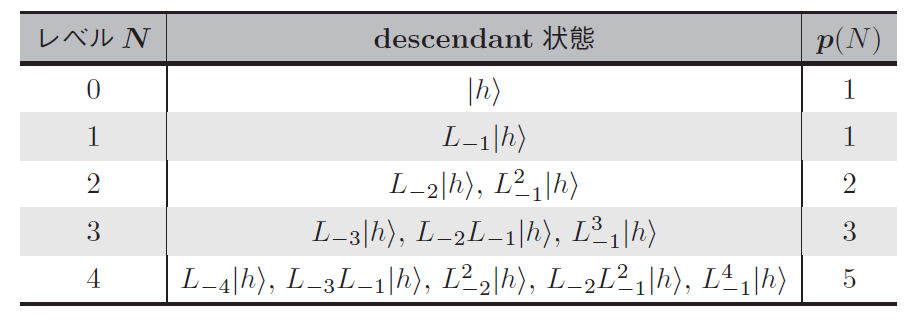
\includegraphics[width=0.6\linewidth]{fig/5.2notag.png}
\end{figure*}

$p(N) $是$ N$ 的拆分数,可通过对无穷乘积
\begin{equation}
	P(q)=\prod_{n=1}^{\infty}\left(1-q^{n}\right)
\end{equation}
的倒数作Taylor展开:
\begin{equation}
	\prod_{n=1}^{\infty}\left(1-q^{n}\right)^{-1}=\sum_{n=0}^{\infty} p(n) q^{n}, \quad|q|<1
\end{equation}
来计算。

态$ |\{n\},h\rangle$ 的Hermite共轭是
\begin{equation}
	\langle h,\{n\}|=\langle h| L_{\{n\}}=\langle h| L_{n_{k}} \cdots L_{n_{1}}
\end{equation}

为讨论Verma模 $V_h$ 中内积的正定性,有必要计算次级态间的内积$ \langle h,\{n'\}|\{n\},h\rangle $。由 $|h\rangle $的范数归一化的内积
$$
\frac{\langle h,\{n'\}|\{n\},h\rangle}{\langle h|h\rangle}
$$
称为Shapovarov形式。因为$ |\{n\},h\rangle$ 是Virasoro算符 $L_0 $的本征值为$h+N$($N=\sum_{i=1}^{k} n_{i}$)的本征态,只有同级态间的内积非零。考虑级为 $N$ 的次级态间归一化内积的矩阵
\begin{equation}
	M(c, h)_{N}=\left(\frac{\left\langle h,\left\{n^{\prime}\right\} |\{n\}, h\right\rangle}{\langle h | h\rangle}\right)
\end{equation}
这是一个 $p(N)\times p(N) $矩阵。

在酉的理论中,各级Shapovarov形式都非负。正定时, $V_h$ 是Virasoro代数的不可约表示。在退化表示的情形, $V_h $中存在一个零模态。既然这时 $M(c, h)_{N} $有一个本征值为零的本征态,就可以得到Shapovarov形式非负的一个边界条件。

例如我们计算$ L_{-n}|h\rangle$ ( $n\geq 1 $)的范数,这非负的条件是
\begin{equation}
	\begin{aligned} \left\langle h\left|L_{n} L_{-n}\right| h\right\rangle &= \langle h\left|\left[L_{n}, L_{-n}\right]\right| h \rangle \\ &= \langle h |\left(2 n L_{0}+\frac{c}{12} n\left(n^{2}-1\right)\right) | h \rangle \\ &=\left(2 n h+\frac{c}{12} n\left(n^{2}-1\right)\right)\langle h |h\rangle \geq 0 \end{aligned}
\end{equation}
$n=1 $时,这是
$$
\langle h|L_1L_{-1}|h\rangle=2h\langle h|h\rangle \geq0
$$
如果 $\langle h|h\rangle>0 $,这就意味着$ h\geq 0 $。此外,考虑 $n$ 足够大的情形,如果 $c<0$ ,那么 (5.98) 是负的。因此,酉的CFT必须满足
\begin{equation}
	h \geq 0, \quad c \geq 0
\end{equation}
对前几级,$ M(c, h)_{N}$ 是
\begin{align} M(c, h)_{0} &=1\\ M(c, h)_{1} &=2 h \\ M(c, h)_{2} &=\frac{1}{\langle h | h\rangle}\left(\begin{array}{cc} \langle h,\{2\} |\{2\}, h\rangle & \langle h,\{2\} |\{1,1\}, h\rangle \\ \langle h,\{1,1\} |\{2\}, h\rangle & \langle h,\{1,1\} |\{1,1\}, h\rangle \end{array}\right) \notag\\ &=\left(\begin{array}{cc} 4 h+\frac{c}{2} & 6 h \\ 6 h & 4 h(1+2 h) \end{array}\right)  \end{align}
直接计算Shapovarov形式不容易。$ M(c, h)_{N} $的行列式称为Kac行列式\footnote{V. G. Kac, Lect. Notes. Phys. 94 (1979) 441.},$ N=0,1,2 $时是
\begin{align} &\det M(c, h)_{0}=1 \\ &\det M(c, h)_{1}=2 h \\ &\det M(c, h)_{2}=4 h\left(8 h^{2}+(c-5) h+\frac{c}{2}\right)  \end{align}
$\det M(c, h)_{N}$ 是$ h,c $的多项式。如果令$ \det M(c, h)_{N}=0 $,将得到作为 $c$ 的函数的 $h$ 。 $N=1$ 时得到$ h=0$ , $N=2 $时得到
$$
h=\frac{5-c \pm \sqrt{(c-1)(c-25)}}{16}
$$
这和 (5.30) 中 $h_{1,1},h_{1,2},h_{2,1}$ 的值是一样的。$ h$ 在Kac谱中时,Kac行列式为零。在Verma模$ V_h $中,如果有一个级为 $n(\leq N)$ 的零模态 $|h+n\rangle$ ,那么 $h,c $的值将使行列式为零。$ |h+n\rangle$ 作用上Virasoro算符得到的态
$$
L_{-n_{1}} \cdots L_{-n_{k}}|h+n\rangle, \quad n_{1} \geq \cdots \geq n_{k}\geq 1
$$
也是零模态。级为 $N $的零模态,可以要求$ n_{1}+\cdots+n_{k}=N-n $来这样构造。这些态的数目是$ p(N-n)$ 。也就是说,对应级为 $n$ 的零模态, $M(c, h)_{N} $有 $p(N-n) $个本征值为零。因为对应Kac谱中 $h_{n,m}$ 的是级为 $nm $的零模态, $\det M(c, h)_{N}$ 包含因子 $\left(h-h_{n, m}\right)^{p(N-n m)} $。Kac猜想
\begin{equation}
	\operatorname{det} M(c, h)_{N}=\alpha_{N} \prod_{n m \leq N}\left(h-h_{n, m}\right)^{p(N-n m)}
\end{equation} 
$\alpha_N$ 是一正常数。这个猜想后来被Feigin-Fuchs\footnote{B. L. Feigin and D. B. Fuchs, Funct. Anal. and Appl. 16 (1984) 114, 17 (1983) 241.}证明了。这里令 $\alpha_{-}=\sqrt{\frac{q}{q+1}}$ 将很方便,那么中心荷是
\begin{equation}
	c=1-\frac{6}{q(q+1)}
\end{equation}
取逆得到
\begin{equation}
	q=-\frac{1 \pm \sqrt{\frac{25-c}{1-c}}}{2}
\end{equation}
Kac谱中的 $h_{n,m}$可写成
\begin{equation}
	h_{n, m}=\frac{[(q+1) n-q m]^{2}-1}{4 q(q+1)}
\end{equation}

Kac行列式可能在 $(c,h) $空间中的一处区域内是正的,另一处则是负的。在负的区域, $M(c, h)_{N}$ 有奇数个负本征值,内积不正定。在各级排除掉行列式是负的情形,或者找到一个关于$ c,h $的条件使得行列式非负,就是CFT酉的必要条件。首先,考虑$ c\geq1,h\geq 0 $的情形,如果 $1<c<25$ ,那么$q $有虚部,因而$ h_{n,m} $有虚部( $n\neq m $)或是负的($ n=m $)。所以, $h>0$ 时,$ \det M(c, h)_{N}$ 不会为零。另一方面,$ h$ 很大时,$\det M(c, h)_{N} $是正的,因此 $h>0$ 时行列式总是正的。

如果 $c\geq 25$ ,那么 $-1<q<0$ 。这时 $h_{n,m} $是负的,$ h>0$ 时 $\det M(c, h)_{N}$是正的。如果$ c=1$ ,那么$ h_{n, m}=\frac{(n-m)^{2}}{4}$ ,$ h\geq 0 $时$ \det M(c, h)_{N} $有零点,但总不会是负的。因此,如果 $c\geq1,h\geq 0$ ,从行列式的讨论中得不出理论非酉。

\begin{figure}[h]
	\centering
	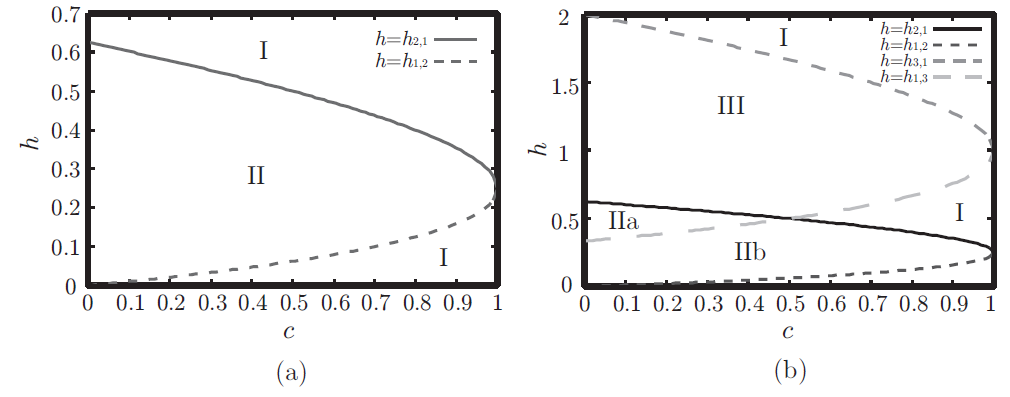
\includegraphics[width=0.7\linewidth]{fig/5.2.png}
	\caption{$(c,h)$平面上的酉区域。(a)级$N=2$,(b)$N=3$。}
\end{figure}

$0<c<1 $时,$Kac$行列式的正负区域由曲线 $h=h_{n, m}(c)$ 分开。这条曲线在 $c=0 $时的值是 $h=\frac{(3 n-2 m)^{2}-1}{24} $, $c=1$ 时的值是 $h=\frac{(n-m)^{2}}{4} $。我们在各级排除掉行列式是负的情形。 $N=1$ 时,这给出$ h\geq 0 $。 $N=2 $时,在图5.2(a)的 $h=h_{2,1}(c) $和 $h=h_{1,2}(c)$ 围起来的区域II中, $\det M(c, h)_{2}<0$ 。在边界上理论可能是酉的。

然后考虑$ N=3 $的情形。可以看到,在图5.2(b)的区域III和IIb中, $\det M(c, h)_{3}<0 $。 $N=2 $时已经排除了区域IIa,那么区域IIa,IIb和III就都被排除了。在边界$ h=h_{1,3} $上,位于区域II中的部分也被排除了。同理,在边界 $h=h_{2,1} $上,区域IIa和III间的线段也被排除了。剩下 $h=h_{2,1}$ 和 $h=h_{1,3}$ 的交点$ (c,h)=(1/2,1/2) $。讨论更高级时不会排除掉这个点,它刚好对应Ising模型。重复这些论证将得到,酉的理论对应$ q=3,4,5,\cdots$ 。这点是由Friedan-Qiu-Shenker\footnote{D. Friedan, Z. a. Qiu and S. H. Shenker, Phys. Rev. Lett. 52 (1984) 1575.}\footnote{D. Friedan, S. H. Shenker and Z. a. Qiu, Commun. Math. Phys. 107 (1986) 535.}\footnote{D. Friedan, Z. a. Qiu and S. H. Shenker, “Conformal Invariance, Unitarity and Two Dimensional Critical Exponents” in Vertex Operators in Mathematical Physics, Springer–Verlag, 1984.}证明的。Goddard-Kent-Olive\footnote{P. Goddard, A. Kent and D. I. Olive, Commun. Math. Phys. 103 (1986) 105.}证明了,这不只是酉的必要条件,也是充分条件。

\section{共形块和单值变换不变性}
4.4节讨论过,四点关联函数具有交叉对称性。本节,我们调查含极小模型中退化初级场的四点关联函数的全局性质。在5.2节,我们推导了含退化初级场的关联函数满足的微分方程,并将含场 $\phi_{(1,2)}$ 的四点关联函数写成超几何级数。考虑到反全纯部分,四点函数$ G_{32}^{10}(x, \bar{x})=\left\langle\phi_{(2,1)}(\infty, \infty) \phi_{1}(1,1) \phi_{2}(x, \bar{x}) \phi_{3}(0,0)\right\rangle$ 是
\begin{equation}
	G_{32}^{10}(x, \bar{x})=|x|^{2 a_{1}+2 a_{2}}|1-x|^{2 b_{1}+2 b_{2}} \sum_{i, j=1}^{2} X_{i j} y_{i}^{(0)}(x) \overline{y_{j}^{(0)}(x)} 
\end{equation}
其中 $a_{1}+a_{2}=h\left(\alpha_{1}-\alpha_{-}\right)-h_{2}-h_{3} $, $b_{1}+b_{2}=h\left(\alpha_{3}-\alpha_{-}\right)-h_{1}-h_{2}$ , $X_{ij}$ 是常数, $y_{1}^{(0)}(x), y_{2}^{(0)}(x) $是超几何微分方程 (5.41) 在$ x=0$ 附近的基本解 (5.46),(5.48) 。这个关联函数的表达式是在 $x=0$ 附近得到的,但关联函数本身定义在除去$ x=0,1,\infty $的复平面上。它的值在给定 $x $处应当是唯一确定的。另一方面,这个微分方程的解有固定奇点$ x=0,1,\infty $,沿绕奇点的路径延拓时会经历带相位因子的变换。解的这个变换称为单值变换。由于物理的要求,关联函数的值在给定 $x$ 处唯一确定, $G_{32}^{10}(x, \bar{x}) $应当在单值变换下不变。

\begin{figure}[h]
	\centering
	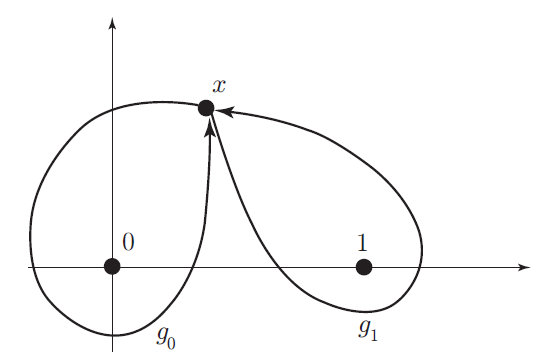
\includegraphics[width=0.6\linewidth]{fig/5.3.png}
	\caption{绕$x=0,1$时经历的单值变换。}
\end{figure}

从点$x$出发,逆时针沿绕$x=0 $的闭合曲线时经历的变换记作$g_0$ ,绕 $x=1$的记作$g_1$,如图5.3。因为绕无穷远点的$g_\infty $由$ g_1g_0 $生成,验证$g_0,g_1$下不变就足够了。

绕$ x=0$一圈,也就是$x \rightarrow x e^{2 \pi i} $, $y_{1}^{(0)}(x), y_{2}^{(0)}(x) $变换为
\begin{equation}
	g_{0}\left(\begin{array}{c} y_{1}^{(0)}(x) \\ y_{2}^{(0)}(x) \end{array}\right)=\left(\begin{array}{cc} 1 & 0 \\ 0 & \omega_{0} \end{array}\right)\left(\begin{array}{l} y_{1}^{(0)}(x) \\ y_{2}^{(0)}(x) \end{array}\right)
\end{equation} 
其中 $\omega_{0}=\exp (2 \pi i(1-\gamma)) $。$ G_{32}^{10}(x, \bar{x})$ 在变换 $g_0 $下不变,要求$ X_{i j}$ 满足
$$
\sum_{i, j} X_{i j}\left(g_{0}\right)_{i k} \overline{\left(g_{0}\right)}_{j l}=X_{k l}
$$
因为$ \left(g_{0}\right)_{i k} $是对角矩阵 $\left(g_{0}\right)_{i i} \delta_{i k}$ ,上式即
$$
		X_{k l}\left(g_{0}\right)_{k k} \overline{\left(g_{0}\right)}_{l l}=X_{k l} 
$$
那么$i\neq j $时$X_{ij}=0 $。因此四点函数可写成
\begin{equation}
	G_{32}^{10}(x, \bar{x})=|x|^{2 a_{1}+2 a_{2}}|1-x|^{2 b_{1}+2 b_{2}} \sum_{i=1}^{2} X_{i i} y_{i}^{(0)}(x) \overline{y_{i}^{(0)}(x)} 
\end{equation}
考虑$x=1$ 附近的单值变换。令$\xi=1-x $, (5.41) 成为
\begin{equation}
	\xi(1-\xi) \frac{d^{2} y}{d \xi^{2}}+(\alpha+\beta+1-\gamma-(\alpha+\beta+1) \xi) \frac{d y}{d \xi}-\alpha \beta y=0
\end{equation} 
那么这时的级数解 $y_{1}^{(1)}(x), y_{2}^{(1)}(x) $相比$ x=0 $附近的,要将 $\alpha,\beta,\gamma$ 换成 $\alpha,\beta,\alpha+\beta+1-\gamma $:
\begin{equation}
	\begin{aligned} &y_{1}^{(1)}(x)=F(\alpha, \beta, 1+\alpha+\beta-\gamma, 1-x) \\ &y_{2}^{(1)}(x)=(1-x)^{\gamma-\alpha-\beta} F(\gamma-\beta, \gamma-\alpha, 1+\gamma-\alpha-\beta, 1-x) \end{aligned}
\end{equation}
对这个解,绕 $x=1$ 一圈,也就是 $1-x \rightarrow(1-x) e^{2 \pi i} $, $y_{1}^{(1)}(x), y_{2}^{(1)}(x)$ 变换为
\begin{equation}
	g_{1}\left(\begin{array}{c} y_{1}^{(1)}(x) \\ y_{2}^{(1)}(x) \end{array}\right)=\left(\begin{array}{cc} 1 & 0 \\ 0 & \omega_{1} \end{array}\right)\left(\begin{array}{l} y_{1}^{(1)}(x) \\ y_{2}^{(1)}(x) \end{array}\right)
\end{equation} 
其中 $\omega_{1}=\exp (2 \pi i(\gamma-\alpha-\beta))$ 。

对无穷远点 $x=\infty $也类似。令$ x=1/\xi$ , $y=\xi^{\alpha} y^{\prime} $, (5.41) 成为
\begin{equation}
	\xi(1-\xi) \frac{d^{2} y^{\prime}}{d \xi^{2}}+(\alpha-\beta+1-(2 \alpha-\gamma+2) \xi) \frac{d y^{\prime}}{d \xi}-\alpha(\alpha-\gamma+1) y^{\prime}=0
\end{equation} 
那么这时的级数解$ y_{1}^{(\infty)}(x), y_{2}^{(\infty)}(x) $相比$ x=0$ 附近的,要将$ \alpha,\beta,\gamma$ 换成 $\alpha,\alpha-\gamma+1,\alpha-\beta+1$:
\begin{equation}
	\begin{aligned} &y_{1}^{(\infty)}(x)=x^{-\alpha} F\left(\alpha, \alpha+1-\gamma, \alpha+1-\beta, \frac{1}{x}\right) \\ &y_{2}^{(\infty)}(x)=x^{-\beta} F\left(\beta, \beta+1-\gamma, \beta+1-\alpha, \frac{1}{x}\right) \end{aligned}
\end{equation}
单值变换是
\begin{equation}
	g_{\infty}\left(\begin{array}{c} y_{1}^{(\infty)}(x) \\ y_{2}^{(\infty)}(x) \end{array}\right)=\left(\begin{array}{cc} e^{-2 \pi i \alpha} & 0 \\ 0 & e^{-2 \pi i \beta} \end{array}\right)\left(\begin{array}{l} y_{1}^{(\infty)}(x) \\ y_{2}^{(\infty)}(x) \end{array}\right)
\end{equation} 
这三点附近的基本解间有关系
\begin{align} &y_{i}^{(0)}(x)=\sum_{j=1}^{2} a_{i j} y_{j}^{(1)}(x) \\ &y_{i}^{(0)}(x)=\sum_{j=1}^{2} b_{i j} y_{j}^{(\infty)}(x) \end{align}
借助超几何级数的解析延拓公式\footnote{犬井鉄郎,『特殊函数』,岩波全書,1962.}
\begin{align} F(\alpha, \beta, \gamma, x)=& \frac{\Gamma(\gamma) \Gamma(\gamma-\alpha-\beta)}{\Gamma(\gamma-\alpha) \Gamma(\gamma-\beta)} F(\alpha, \beta, 1+\alpha+\beta-\gamma, 1-x) \notag\\ &+\frac{\Gamma(\gamma) \Gamma(\alpha+\beta-\gamma)}{\Gamma(\alpha) \Gamma(\beta)}(1-x)^{\gamma-\alpha-\beta} \\ & \times F(\gamma-\beta, \gamma-\alpha, 1+\gamma-\alpha-\beta, 1-x)\notag\\ F(\alpha, \beta, \gamma, x)=& \frac{\Gamma(\gamma) \Gamma(\beta-\alpha)}{\Gamma(\beta) \Gamma(\gamma-\alpha)}(-x)^{-\alpha} F\left(\alpha, 1+\alpha-\gamma, 1+\alpha-\beta, \frac{1}{x}\right) \notag\\ &+\frac{\Gamma(\gamma) \Gamma(\alpha-\beta)}{\Gamma(\alpha) \Gamma(\gamma-\beta)}(-x)^{-\beta} F\left(\beta, 1+\beta-\gamma, 1+\beta-\alpha, \frac{1}{x}\right) \end{align}
我们得到变换矩阵$ a_{ij},b_{ij} $是
\begin{align} &\left(a_{i j}\right)=\left(\begin{array}{cc} \frac{\Gamma(\gamma) \Gamma(\gamma-\alpha-\beta)}{\Gamma(\gamma-\alpha) \Gamma(\gamma-\beta)} & \frac{\Gamma(\gamma) \Gamma(\alpha+\beta-\gamma)}{\Gamma(\alpha) \Gamma(\beta)} \\ \frac{\Gamma(2-\gamma) \Gamma(\gamma-\alpha-\beta)}{\Gamma(1-\alpha) \Gamma(1-\beta)} & \frac{\Gamma(2-\gamma) \Gamma(\alpha+\beta-\gamma)}{\Gamma(\alpha-\gamma+1) \Gamma(\beta-\gamma+1)} \end{array}\right) \\ &\left(b_{i j}\right)=\left(\begin{array}{cc} \frac{\Gamma(\gamma) \Gamma(\beta-\alpha)}{\Gamma(\beta) \Gamma(\gamma-\alpha)} e^{-\pi i \alpha} & \frac{\Gamma(\gamma) \Gamma(\alpha-\beta)}{\Gamma(\alpha) \Gamma(\gamma-\beta)} e^{-\pi i \beta} \\ \frac{\Gamma(2-\gamma) \Gamma(\beta-\alpha)}{\Gamma(\beta-\gamma+1) \Gamma(1-\alpha)} e^{-\pi i(\alpha-\gamma+1)} &\frac{\Gamma(2-\gamma) \Gamma(\alpha-\beta)}{\Gamma(\alpha-\gamma+1) \Gamma(1-\beta)} e^{-\pi i(\beta-\gamma+1)} \end{array}\right)\end{align}
(5.119) 代入 (5.112) ,得到$ G_{32}^{10}(x, \bar{x})$ 在$ x=1$ 附近的级数表示:
\begin{align} &G_{32}^{10}(x, \bar{x})=|x|^{2 a_{1}+2 a_{2}}|1-x|^{2 b_{1}+2 b_{2}} \sum_{i, j=1}^{2} X_{i j}^{1} y_{i}^{(1)}(x) \overline{y_{j}^{(1)}(x)} \\ &X_{i j}^{1}=\sum_{k=1}^{2} X_{k k} a_{k i} \bar{a}_{k j} \end{align}

关联函数在 $g_1 $下不变,要求$ X_{i j}^{1} $的非对角项$ X_{12}^{1} $为零,那么
$$
X_{11} a_{11} \bar{a}_{12}+X_{22} a_{21} \bar{a}_{22}=0
$$
换言之
\begin{equation}
	\begin{aligned} \frac{X_{11}}{X_{22}} &=-\frac{a_{21} \bar{a}_{22}}{a_{11} \bar{a}_{12}} \\ &=-\frac{\Gamma(2-\gamma)^{2} \Gamma(\alpha) \Gamma(\beta) \Gamma(\gamma-\alpha) \Gamma(\gamma-\beta)}{\Gamma(\gamma)^{2} \Gamma(1-\alpha) \Gamma(1-\beta) \Gamma(\alpha-\gamma+1) \Gamma(\beta-\gamma+1)} \end{aligned}
\end{equation} 
因此四点函数可写成
\begin{equation}
	\begin{aligned} G_{32}^{10}(x, \bar{x})=&|x|^{2 h\left(\alpha_{1}-\alpha_{-}\right)-2 h_{2}-2 h_{3}}|1-x|^{2 h\left(\alpha_{3}-\alpha_{-}\right)-2 h_{1}-2 h_{2}} \\ & \times \lambda\left(\frac{\Gamma(\alpha) \Gamma(\beta) \Gamma(\gamma-\alpha) \Gamma(\gamma-\beta)}{\Gamma(\gamma)^{2}}\left|y_{1}^{(0)}(x)\right|^{2}\right.\\&\left.-\frac{\Gamma(1-\alpha) \Gamma(1-\beta) \Gamma(1-\gamma+\alpha) \Gamma(1-\gamma+\beta)}{\Gamma(2-\gamma)^{2}}\left|y_{2}^{(0)}(x)\right|^{2}\right) \end{aligned}
\end{equation} 
其中 $\lambda$ 是常数。$ G_{32}^{10}(x, \bar{x}) $在 $x=1 $附近可写成
\begin{equation}
	\begin{aligned} G_{32}^{10}(x, \bar{x})=&|x|^{2 h\left(\alpha_{1}-\alpha_{-}\right)-2 h_{2}-2 h_{3}}|1-x|^{2 h\left(\alpha_{3}-\alpha_{-}\right)-2 h_{1}-2 h_{2}} \\ & \times \lambda^{\prime}\left(\frac{\Gamma(\gamma-\alpha-\beta)^{2}}{\Gamma(1-\alpha) \Gamma(1-\beta) \Gamma(\gamma-\alpha) \Gamma(\gamma-\beta)}\left|y_{1}^{(1)}(x)\right|^{2}\right.\\&\left.-\frac{\Gamma(\alpha+\beta-\gamma)^{2}}{\Gamma(\alpha) \Gamma(\beta) \Gamma(1+\alpha-\gamma) \Gamma(1+\beta-\gamma)}\left|y_{2}^{(1)}(x)\right|^{2}\right) \end{aligned}
\end{equation} 
其中
\begin{equation}
	\begin{aligned} \lambda^{\prime}=& \lambda \frac{\Gamma(\alpha) \Gamma(1-\alpha) \Gamma(\beta) \Gamma(1-\beta)}{\Gamma(\gamma) \Gamma(1-\gamma)} \\ & \times \frac{\Gamma(\gamma-\alpha) \Gamma(1+\alpha-\gamma) \Gamma(\gamma-\beta) \Gamma(1+\beta-\gamma)}{\Gamma(\gamma-\alpha-\beta) \Gamma(1+\alpha+\beta-\gamma)} \end{aligned} 
\end{equation}

计算关联函数的具体例子,有描述Ising模型\footnote{A. A. Belavin, A. M. Polyakov and A. B. Zamolodchikov, Nucl. Phys. B 241 (1984) 333.}和Yang-Lee边界奇点\footnote{J. L. Cardy, Phys. Rev. Lett. 54 (1985) 1345.}的极小模型。Yang-Lee边界奇点对应CFT的中心荷是 $c=-22/5$ ,含恒等算符$ \boldsymbol{I}$ 和共形权是$ (-1/5,-1/5)$ 的初级场$ \varphi=\phi_{(1,2)}$ 。这个模型中非平凡的四点函数是
$$
\left\langle\varphi\left(z_{1}, \bar{z}_{1}\right) \varphi\left(z_{2}, \bar{z}_{2}\right) \varphi\left(z_{3}, \bar{z}_{3}\right) \varphi\left(z_{4}, \bar{z}_{4}\right)\right\rangle
$$
这时 $t=2/5 $, $\alpha_{1}=\alpha_{2}=\alpha_{3}=\alpha_{+}+2 \alpha_{-}$ ,我们有
\begin{align} &a_1=b_1=0,\quad a_2=b_2=2/5\\ &\alpha=4/5,\quad \beta=3/5,\quad \gamma=6/5 \end{align}
因此
\begin{equation}
	\begin{aligned} G_{\varphi \varphi}^{\varphi \varphi}(x, \bar{x})=\lambda|x|^{\frac{4}{5}}|1-x|^{\frac{4}{5}} &\left\{N_{1}\left|F\left(\frac{4}{5}, \frac{3}{5}, \frac{6}{5}, x\right)\right|^{2}\right.\\&\left.+N_{2}\left|x^{-\frac{1}{5}} F\left(\frac{3}{5}, \frac{2}{5}, \frac{4}{5}, x\right)\right|^{2}\right\} \end{aligned} 
\end{equation}
其中
\begin{align} &N_{1}=\frac{\Gamma\left(4/5\right) \Gamma\left(3/5\right)^{2} \Gamma\left(2/5\right)}{\Gamma\left(6/5\right)} \\ &N_{2}=-\frac{\Gamma\left(1/5\right) \Gamma\left(2/5\right)^{2} \Gamma\left(3/5\right)}{\Gamma\left(4/5\right)^{2}} \end{align}

接着考虑Ising模型,它含恒等算符 $\boldsymbol{I}$($h=\bar{h}=0$),自旋算符$ \sigma(z, \bar{z})=\phi_{(1,2)}(z, \bar{z})$( $h=\bar{h}=1/16$)和能量密度算符$\epsilon(z, \bar{z})=\phi_{(2,1)}(z, \bar{z})$($h=\bar{h}=1/2 $)。考虑自旋算符的四点函数
$$
\left\langle\sigma\left(z_{0}, \bar{z}_{0}\right) \sigma\left(z_{1}, \bar{z}_{1}\right) \sigma\left(z_{2}, \bar{z}_{2}\right) \sigma\left(z_{3}, \bar{z}_{3}\right)\right\rangle
$$
这时 $h_{0}=h_{1}=h_{2}=h_{3} =1/16 $,我们有
\begin{equation}
	\begin{aligned} &a_{1}=b_{1}=0, \quad a_{2}=b_{2}=-1/8 \\ &\alpha=-1/4,\quad \beta=1/4,\quad \gamma=1/2
	 \end{aligned}
\end{equation}
于是关联函数可写成
\begin{equation}
	\left\langle\sigma\left(z_{0}, \bar{z}_{0}\right) \sigma\left(z_{1}, \bar{z}_{1}\right) \sigma\left(z_{2}, \bar{z}_{2}\right) \sigma\left(z_{3}, \bar{z}_{3}\right)\right\rangle=\left|\frac{z_{13} z_{02}}{z_{01} z_{23} z_{12} z_{03}}\right|^{\frac{1}{4}} F(x, \bar{x})
\end{equation}
$F(x, \bar{x}) $满足微分方程
\begin{equation}
	x(1-x) \frac{d^{2} F}{d x^{2}}+\left(\frac{1}{2}-x\right) \frac{d F}{d x}+\frac{1}{16} F=0
\end{equation}
令$ x=\sin^2\theta $,这成为
$$
\left(\frac{d^{2}}{d \theta^{2}}+\frac{1}{4}\right) F=0
$$
解得
\begin{equation}
	F_{1}=\cos \frac{\theta}{2}=\frac{1}{2} \sqrt{1+\sqrt{1-x}}, \quad F_{2}=\sin \frac{\theta}{2}=\frac{1}{2} \sqrt{1-\sqrt{1-x}}
\end{equation}
$F(x, \bar{x})$ 可写成$ F_i,\bar{F}_j $的组合:
\begin{equation}
	F(x, \bar{x})=u_{11} F_{1} \bar{F}_{1}+u_{22} F_{2} \bar{F}_{2}+u_{12} F_{1} \bar{F}_{2}+u_{21} F_{2} \bar{F}_{1}
\end{equation} 
绕$ x=0,1,\infty $一圈经历的单值变换是
\begin{align} &F_{1} \rightarrow F_{1}, \quad F_{2} \rightarrow e^{\pi i} F_{2}, \quad x=0\quad \\ &F_{1} \rightarrow F_{2}, \quad F_{2} \rightarrow F_{1}, \quad x=1\quad\\ &F_{1} \rightarrow e^{-\pi i} F_{1}, \quad F_{2} \rightarrow e^{-\pi i} F_{2}, \quad x=\infty\quad  \end{align}
不变性要求 $u_{11}=u_{22} $, $u_{12}=u_{21}=0$ ,因此有
\begin{equation}
	\begin{aligned} F(x, \bar{x})=\lambda\left( \sqrt{1+\sqrt{1-x}} \sqrt{1+\sqrt{1-\bar{x}}}+\sqrt{1-\sqrt{1-x}} \sqrt{1-\sqrt{1-\bar{x}}}\right) \end{aligned}
\end{equation}

\section{四点函数和OPE系数}
上节展示了,含退化初级场$ \phi_{(1,2)}$ 的四点关联函数可写成超几何级数。本节,我们从退化初级场的四点函数
\begin{equation}
	\left\langle\phi_{(1,2)}(\infty, \infty) \phi_{\left(n_{1}, m_{1}\right)}(1,1) \phi_{\left(n_{2}, m_{2}\right)}(x, \bar{x}) \phi_{\left(n_{3}, m_{3}\right)}(0,0)\right\rangle 
\end{equation}
中,提取有关退化初级场OPE系数的信息。

(5.145) 中令$ x $趋于零,用OPE
\begin{equation}
\begin{aligned} \phi_{\left(n_{2}, m_{2}\right)}(x, \bar{x}) \phi_{\left(n_{3}, m_{3}\right)}(0,0)=& \sum_{(n, m)} C_{\left(n_{2}, m_{2}\right)\left(n_{3}, m_{3}\right)}^{(n, m)}|x|^{2 h_{n, m}-2 h_{n_{2},m_2}-2 h_{n_{3},m_3}} \\ & \times\left(\phi_{(n, m)}(0,0)+\cdots\right) \end{aligned}
\end{equation} 
将关联函数展开成
\begin{equation}
	\begin{aligned} &\sum_{(n, m)} C_{\left(n_{2}, m_{2}\right)\left(n_{3}, m_{3}\right)}^{(n, m)}|x|^{2 h_{n,m}-2 h_{n_{2}, m_{2}}-2 h_{n_{3}, m_{3}}} \\ &\times\left\langle\phi_{(1,2)}(\infty, \infty) \phi_{\left(n_{1}, m_{1}\right)}(1,1) \phi_{(n, m)}(0,0)\right\rangle+\cdots \end{aligned}
\end{equation} 
两点和三点函数的归一化条件选为
\begin{align} &\left\langle\phi_{(n_1, m_1)}\left(z_{1}, \bar{z}_{1}\right) \phi_{\left(n_2, m_2\right)}\left(z_{2}, \bar{z}_{2}\right)\right\rangle=\delta_{n_{1}, n_{2}} \delta_{m_{1}, m_{2}}\left|z_{12}\right|^{-4 h_{n_{1},m_1}}\\ &\left\langle\phi_{\left(n_{1}, m_{1}\right)}\left(z_{1}, \bar{z}_{1}\right) \phi_{\left(n_{2}, m_{2}\right)}\left(z_{2}, \bar{z}_{2}\right) \phi_{\left(n_{3}, m_{3}\right)}\left(z_{3}, \bar{z}_{3}\right)\right\rangle \notag\\ &=C_{\left(n_{1}, m_{1}\right)\left(n_{2}, m_{2}\right)\left(n_{3}, m_{3}\right)}\left|z_{12}\right|^{2 h_{3}-2 h_{1}-2 h_{2}}\left|z_{23}\right|^{2 h_{1}-2 h_{2}-2 h_{3}}\left|z_{13}\right|^{2 h_{2}-2 h_{1}-2 h_{3}} 
\end{align}
其中$ h_{i}=h_{n_{i}, m_{i}}$ ( $i=1,2,3 $)。 $C_{\left(n_{1}, m_{1}\right)\left(n_{2}, m_{2}\right)\left(n_{3}, m_{3}\right)} $关于 $(n_i,m_i) $是对称的。取$ \phi_{\left(n_{1}, m_{1}\right)}$ 和 $\phi_{\left(n_{2}, m_{2}\right)} $的OPE,并用两点函数的归一化条件,可以得到 $C_{\left(n_{1}, m_{1}\right)\left(n_{2}, m_{2}\right)\left(n_{3}, m_{3}\right)}=C_{\left(n_{1}, m_{1}\right)\left(n_{2}, m_{2}\right)}^{\left(n_{3}, m_{3}\right)} $。注意,如果含恒等算符 $\phi_{(1,1)}$ ,那么 (5.148) 给出 $C_{\left(n_{2}, m_{2}\right)\left(n_{3}, m_{3}\right)}^{(1,1)}=\delta_{n_{2}, n_{3}} \delta_{m_{2}, m_{3}}$ 。
特别地,三点$ (z_1,z_2,z_3)$ 选成$ (\infty, 1,0) $,使用同 (4.65) 一样的定义,可以得到 (5.147) 中的三点函数就是OPE系数本身:
\begin{equation}
\left\langle\phi_{(1,2)}(\infty, \infty) \phi_{\left(n_{1}, m_{1}\right)}(1,1) \phi_{(n, m)}(0,0)\right\rangle=C_{(1,2)\left(n_{1}, m_{1}\right)(n, m)}
\end{equation} 
根据融合规则,它的值仅当$ (n, m)=\left(n_{1}, m_{1} \pm 1\right) $时非零。因此 (5.147) 等于
\begin{equation}
	\sum_{l=\pm 1} C_{\left(n_{2}, m_{2}\right)\left(n_{3}, m_{3}\right)}^{\left(n_{1}, m_{1}+l\right)} C_{(1,2)\left(n_{1}, m_{1}\right)}^{\left(n_{1}, m_{1}+l\right)}|x|^{2 h_{n_1, m_1+l}-2 h_{n_{2}, m_{2}}-2 h_{n_{3}, m_{3}}}
\end{equation}
与关联函数的超几何级数表达式 (5.128) 比对。在 (5.151) 中,$ l=-1 $项对应 (5.128) 第一项,$ l=+1 $项则对应第二项,于是得到
\begin{align} C_{\left(n_{2}, m_{2}\right)\left(n_{3}, m_{3}\right)}^{\left(n_{1}, m_{1}-1\right)} C_{(1,2)\left(n_{1}, m_{1}\right)}^{\left(n_{1}, m_{1}-1\right)}=& \lambda \frac{\Gamma(\alpha) \Gamma(\beta) \Gamma(\gamma-\alpha) \Gamma(\gamma-\beta)}{\Gamma(\gamma)^{2}} \\ C_{\left(n_{2}, m_{2}\right)\left(n_{3}, m_{3}\right)}^{\left(n_{1}, m_{1}+1\right)} C_{(1,2)\left(n_{1}, m_{1}\right)}^{\left(n_{1}, m_{1}+1\right)}=&-\lambda \Gamma(1-\alpha) \Gamma(1-\beta) \notag\\ & \times \frac{\Gamma(1-\gamma+\alpha) \Gamma(1-\gamma+\beta)}{\Gamma(2-\gamma)^{2}} \end{align}
其中
\begin{align} &\alpha=\frac{1}{2}\left(1+n_{1}+n_{2}+n_{3}-t\left(m_{1}+m_{2}+m_{3}\right)\right)\\ &\beta=\frac{1}{2}\left(1+n_{1}-n_{2}+n_{3}-t\left(m_{1}-m_{2}+m_{3}\right)\right)\\ &\gamma=1+n_{1}-m_{1} t \end{align}

例如,考虑初级场都是 $\phi_{(1,2)}$ ,即 $\left(n_{i}, m_{i}\right)=(1,2) $的情形。归一化给出$ C_{(1,2)(1,2)}^{(1,1)}=1$ ,代入 (5.152) 可求出$ \lambda$ ,于是由 (5.153) 得到
\begin{equation}
	\begin{aligned} C_{(1,2)(1,2)}^{(1,3)} &=\frac{\Gamma(2-2 t)}{\Gamma(2 t)}(-\gamma(t) \gamma(-1+3 t))^{\frac{1}{2}} \\ &=\frac{\Gamma(2-2 t)}{\Gamma(2 t)}\left(-\frac{\gamma(t)^{3}}{\gamma(3 t-1)}\right)^{\frac{1}{2}} \frac{\gamma(1-t)}{\gamma(2-3 t)} \end{aligned} 
\end{equation}
这里, $C_{(1,2)(1,2)}^{(1,3)} $选取正的,
\begin{equation}
	\gamma(x)=\frac{\Gamma(x)}{\Gamma(1-x)}
\end{equation}
$\gamma(x) $满足 $\gamma(x) \gamma(1-x)=1 $。

接着考虑 $\left(n_{1}, m_{1}\right)=(1,2) $, $\left(n_{2}, m_{2}\right)=\left(n_{3}, m_{3}\right)=(n, m) $的情形,这时四点函数是
\begin{equation}
	\left\langle\phi_{(1,2)}(\infty, \infty) \phi_{(1,2)}(1,1) \phi_{(n, m)}(x, \bar{x}) \phi_{(n, m)}(0,0)\right\rangle
\end{equation}
$\alpha=1+n-t(m+1)$, $\beta=1-t$ , $\gamma=2-2 t $。归一化给出 (5.152) 左边是 1 ,那么
\begin{equation}
\lambda=\frac{\Gamma(2-2 t)^{2}}{\Gamma(1+n-t(m+1)) \Gamma(1-n-t(1-m)) \Gamma(1-t)^2}
\end{equation}
(5.153) 左边是$ C_{(n, m)(n, m)}^{(1,3)} C_{(1,2)(1,2)}^{(1,3)} $,代入 (5.157) 得到
\begin{equation}
	C_{(n, m)(n, m)}^{(1,3)}=\frac{\Gamma(2-2 t)}{\Gamma(2 t)}\left(-\frac{\gamma(t)^{3}}{\gamma(3 t-1)}\right)^{\frac{1}{2}} \frac{\gamma(-n+t(m+1))}{\gamma(1+n-t(m+1))}
\end{equation}

考虑四点函数 (5.159) 在 $x\to 1$ 时的极限,我们得到OPE系数间的另一条关系。这时取 $\phi_{(1,2)}(1,1) 和 \phi_{(n, m)}(x, \bar{x}) $的OPE, (5.159) 等于
\begin{equation}
	\sum_{l=\pm 1} C_{(1,2)(n, m)}^{(n, m+l)} C_{(1,2)(n, m)}^{(n, m+l)}|x-1|^{2 h_{n, m+l}-2 h_{1,2}-2 h_{n, m}}+\cdots 
\end{equation}
与 (5.129) 比对得到
\begin{align} &C_{(1,2)(n, m)}^{(n, m-1)} C_{(1,2)(n, m)}^{(n, m-1)}=\lambda^{\prime} \frac{\Gamma(\gamma-\alpha-\beta)^{2}}{\Gamma(1-\alpha) \Gamma(1-\beta) \Gamma(\gamma-\alpha) \Gamma(\gamma-\beta)}\\ &C_{(1,2)(n, m)}^{(n, m+1)} C_{(1,2)(n, m)}^{(n, m+1)}=-\lambda^{\prime} \frac{\Gamma(\alpha+\beta-\gamma)^{2}}{\Gamma(\alpha) \Gamma(\beta) \Gamma(1+\alpha-\gamma) \Gamma(1+\beta-\gamma)} \end{align}
代入 $\alpha,\beta,\gamma $的值得到OPE系数
\begin{align} &C_{(1,2)(n, m)}^{(n, m-1)}=\left(\frac{\gamma(2-2 t) \gamma(-n+t m))}{\gamma(1-t) \gamma(1-n+t(m-1))}\right)^{\frac{1}{2}} \\ &C_{(1,2)(n, m)}^{(n, m+1)}=\left(\frac{\gamma(2-2 t) \gamma(n-t m))}{\gamma(1-t) \gamma(1+n+t(m+1))}\right)^{\frac{1}{2}} \end{align}

例如,在Yang-Lee边界奇点的情形,$ t=2/5$ , $\varphi=\phi_{(1,2)}=\phi_{(1,3)}$ 间的OPE系数 (5.157) 是
\begin{equation}
	C_{\varphi \varphi}^{\varphi}=\frac{i}{5} \frac{\Gamma\left(1/5\right)^2}{\Gamma\left(4/5\right) \Gamma\left(3/5\right)}\left(\frac{\sqrt{5}-1}{2}\right)^{\frac{1}{2}}
\end{equation}
那么OPE是
\begin{equation}
	\varphi(z, \bar{z}) \varphi(0,0)=C_{\varphi \varphi}^{\varphi}|z|^{\frac{2}{5}} \varphi(0,0)+\cdots
\end{equation}
$C_{\varphi \varphi}^{\varphi} $是纯虚数,说明CFT非酉。

在Ising模型的情形,$ \sigma=\phi_{(1,2)}$ , $\epsilon=\phi_{(1,3)} $, $t=3/4$ , (5.157) 是
\begin{equation}
	C_{\sigma \sigma}^{\epsilon}=\frac{1}{2}
\end{equation} 
那么$ \sigma(z, \bar{z})$ 间的OPE是
\begin{equation}
	\sigma(z, \bar{z}) \sigma(0,0) \models|z|^{-\frac{1}{4}}(\boldsymbol{I}(0,0)+\cdots)+\frac{1}{2}|z|^{\frac{3}{4}}(\epsilon(0,0)+\cdots)
\end{equation}

知道了一般退化初级场的四点关联函数,就能具体计算OPE系数。这样的话,需要知道一般零模场满足的微分方程,作为它的解的共形块,和共形块单值变换不变的表达式。使用Dotsenko-Fateev方法\footnote{V. S. Dotsenko and V. A. Fateev, Nucl. Phys. B 240 (1984) 312.}\footnote{V. S. Dotsenko and V. A. Fateev, Nucl. Phys. B 251 (1985) 691.}\footnote{V. S. Dotsenko and V. A. Fateev, Phys. Lett. B 154 (1985) 291.}\footnote{V. S. Dotsenko, Adv. Stud. Pure. Math. 16 (1988) 123.},直接求出共形块的积分表示,就能得到一般四点函数的形式,从而具体计算OPE系数。

\section{Kac谱和自由场}
因为极小模型的中心荷小于1,不直接对应自由玻色子CFT( $c=1 $)。标量场同世界面曲率结合的话,自由玻色系统的中心荷$ c $可以偏离1。在一般的二维度规 $g_{\mu\nu}$ 下,这样的理论作用量是
\begin{equation}
	S=\frac{1}{8 \pi} \int d^{2} x \sqrt{g}\left(g^{\mu \nu} \partial_{\mu} \varphi \partial_{\nu} \varphi+i Q R \varphi\right)
\end{equation} \quad \quad (5.171)
其中, $g=\operatorname{det}\left(g_{\mu \nu}\right) $, $R $是标量曲率, $Q$ 是常数。标量场平移 $\varphi \rightarrow \varphi+\varphi_{0}$ ( $\varphi_0$ 是常数)下,作用量变化了
$$
\delta S=\frac{i Q \varphi_{0}}{8 \pi} \int d^{2} x \sqrt{g} R
$$
二维曲面是亏格(洞的数目)为 h 的Riemann面时,Gauss-Bonnet定理给出
\begin{equation}
	\int d^{2} x \sqrt{g} R=8 \pi(1-h)
\end{equation} 
对球面,$ h=0$ ,$ \delta S=i Q \varphi_{0}$ ,于是 (3.114) 变为
\begin{equation}
	\begin{aligned} &\left\langle e^{i \sqrt{2} \alpha_{1} \varphi\left(z_{1}, \bar{z}_{1}\right)} \ldots e^{i \sqrt{2} \alpha_{N} \varphi\left(z_{N}, \bar{z}_{N}\right)}\right\rangle \\ =& e^{\left(i \sqrt{2} \sum_{i=1}^{N} \alpha_{i}-i Q\right) \varphi_{0}}\left\langle e^{i \sqrt{2} \alpha_{1} \varphi\left(z_{1}, \bar{z}_{1}\right)} \cdots e^{i \sqrt{2} \alpha_{N} \varphi\left(z_{N}, \bar{z}_{N}\right)}\right\rangle \end{aligned} 
\end{equation}
因此,只有
\begin{equation}
	\sum_{i=1}^{N} \alpha_{i}=\frac{1}{\sqrt{2}} Q
\end{equation} 
时,这个关联函数非零。

度规是
\begin{equation}
	d s^{2}=\rho d z d \bar{z}, \quad g_{z \bar{z}}=\frac{1}{2} \rho, \quad g_{z z}=g_{\bar{z} \bar{z}}=0
\end{equation}
时,标量曲率是
\begin{equation}
	R=\rho^{-1}\left(-4 \partial_{z} \partial_{\bar{z}} \log \rho\right)
\end{equation}
于是
$$
\sqrt{g} R=-2 \partial_{z} \partial_{\bar{z}} \log \rho
$$
对度规为 $d s^{2}=d z d \bar{z} $的复平面, $\sqrt{g} R=0 $。另一方面, $z=\infty $时,在原点附近作坐标变换$ w=1/z$ ,度规成为 $w^{-2} \bar{w}^{-2} d w d \bar{w} $, $\sqrt{g} R \sim \delta^{2}(0)$ 。这相当于,Riemann球面上 $z=\infty $处有电荷$ -Q $, (5.174) 表达电荷中性条件。 $Q $常称为背景荷。\footnote{接下来的计算类似\href{https://zhuanlan.zhihu.com/p/150578081}{[BBS] 3.6 线性胀子真空和非临界弦}}

从作用量可推出,这个CFT的能动张量是
\begin{equation}
	T(z)=-\frac{1}{2}:(\partial \varphi)^{2}:+i \frac{Q}{2} \partial^{2} \varphi 
\end{equation}
计算 $T(z)$ 间的OPE,将得到额外的$ (z-w)^{-4} $项:
\begin{equation}
	\left(i \frac{Q}{2}\right)^{2} \partial^{2} \varphi(z) \partial^{2} \varphi(w)=\frac{-\frac{3 Q^{2}}{2}}{(z-w)^{4}}+\cdots 
\end{equation}
于是中心荷是
\begin{equation}
	c=1-3 Q^{2} 
\end{equation}

计算 $T(z)$ 和顶点算符$ V_{\beta}(z)=: e^{i \sqrt{2} \beta \varphi(z)}:$ 间的OPE,将得到额外的$ (z-w)^{-2} $项:
\begin{equation}
	\frac{i Q}{2} \partial^{2} \varphi(z) V_{\beta}(w)=\frac{\frac{i Q}{2} i \sqrt{2} \beta}{(z-w)^{2}} V_{\beta}(w)+\cdots 
\end{equation}
于是它的共形权是
\begin{equation}
	h=\beta^{2}-\frac{Q}{\sqrt{2}} \beta
\end{equation} 

现在与5.1节讨论过的Kac谱方程 (5.27),(5.29) 比对。首先,取$ Q=2 \sqrt{2} \alpha_{0} $比较方便,我们有
\begin{align} &c=1-24 \alpha_{0}^{2}\\ &h=\beta^{2}-2 \beta \alpha_{0}=\left(\beta-\alpha_{0}\right)^{2}-\alpha_{0}^{2} \end{align}
于是由 (5.27) 知 $\alpha_{+}+\alpha_{-} $对应 $\alpha_0$ ,由 (5.29) 知$ n \alpha_{+}+m \alpha_{-}$ 对应 $\beta$ ,具体来说是
\begin{align} &\alpha_{0}=\frac{1}{2}\left(\alpha_{+}+\alpha_{-}\right) \\ &\beta=\beta_{n, m} \equiv \frac{1}{2}(1-n) \alpha_{+}+\frac{1}{2}(1-m) \alpha_{-}\end{align}
由 (5.183) 可知, $V_{\beta}(z) $和 $V_{2 \alpha_{0}-\beta}(z)$ 的共形权相等,我们引入记号
\begin{equation}
	\bar{\beta}_{n, m}=2 \alpha_{0}-\beta_{n, m}=\frac{1}{2}(1+n) \alpha_{+}+\frac{1}{2}(1+m) \alpha_{-} 
\end{equation}
那么,Kac谱中共形权$h_{n,m}$的初级场$\phi_{(n, m)}(z) $,对应顶点算符 $V_{\beta_{n, m}}(z) $和$ V_{\bar{\beta}_{n, m}}(z) $。

\section{关联函数的自由场表示}
如何基于上节极小模型和自由场的对应,来表示初级场的关联函数呢?背景荷的效果,相当于$ z=\infty $处有带荷 $-2\alpha_0 $的顶点算符 $V_{-2 \alpha_{0}}(\infty) $。这时顶点算符 $V_{\beta_{1}}\left(z_{1}\right), \cdots, V_{\beta_{N}}\left(z_{N}\right) $的关联函数,等价于这样一个含 $V_{-2 \alpha_{0}}(\infty)$ 的 $N+1$ 点函数,像 (4.65) 那样定义为
\begin{equation}
	\begin{aligned} \left\langle V_{\beta_{1}}\left(z_{1}\right) \cdots V_{\beta_{N}}\left(z_{N}\right)\right\rangle_{-2 \alpha_{0}} &=\left\langle V_{\beta_{1}}\left(z_{1}\right) \cdots V_{\beta_{N}}\left(z_{N}\right) V_{-2 \alpha_{0}}(\infty)\right\rangle \\ & \equiv \lim _{z \rightarrow \infty} z^{8 \alpha_{0}^{2}}\left\langle V_{\beta_{1}}\left(z_{1}\right) \cdots V_{\beta_{N}}\left(z_{N}\right) V_{-2 \alpha_{0}}(z)\right\rangle \end{aligned} 
\end{equation}
左边的 $\langle\cdots\rangle_{-2 \alpha_{0}}$ ,指关联函数是在背景荷 $Q=-2 \sqrt{2} \alpha_{0} $下计算的。简单起见,将$ \langle\cdots\rangle_{-2 \alpha_{0}}$ 写成$ \langle\langle\cdots\rangle\rangle$ 。右边的关联函数是在无背景荷时计算的。只有
\begin{equation}
	\sum_{i=1}^{N} \beta_{i}=2 \alpha_{0} 
\end{equation}
时,这个关联函数非零。

例如,由 (3.111) ,我们有两点函数
\begin{equation}
	\left\langle\left\langle V_{\beta}(z) V_{2 \alpha_{0}-\beta}(w)\right\rangle\right\rangle=(z-w)^{2 \beta\left(2 \alpha_{0}-\beta\right)}=\frac{1}{(z-w)^{2 h}}
\end{equation}
其中$ h=\beta^{2}-2 \beta \alpha_{0}$ 。这等价于Kac谱中相应初级场的两点函数。上式对任意$ \beta $都成立,但如果换成$\left\langle\left\langle V_{\beta}(z) V_{\beta}(w)\right\rangle\right\rangle$ ,就只有 $2 \beta=2 \alpha_{0}$ 时非零。自由场顶点算符的关联函数要等价于极小模型中初级场的关联函数的话,电荷中性条件至关重要。

四点函数呢?我们想表示共形权为$ h $的初级场 $\phi_{h}(z)$ 的四点函数 $\left\langle\phi_{h}\left(z_{1}\right) \phi_{h}\left(z_{2}\right) \phi_{h}\left(z_{3}\right) \phi_{h}\left(z_{4}\right)\right\rangle $,考虑这样一些自由场顶点算符 $V_{\beta}(z) 和 V_{2 \alpha_{0}-\beta}(z)$ 的四点函数:
\begin{align} &\left\langle\left\langle V_{\beta}\left(z_{1}\right) V_{\beta}\left(z_{2}\right) V_{\beta}\left(z_{3}\right) V_{\beta}\left(z_{4}\right)\right\rangle\right\rangle \\ &\left\langle\left\langle V_{\beta}\left(z_{1}\right) V_{\beta}\left(z_{2}\right) V_{\beta}\left(z_{3}\right) V_{2 \alpha_{0}-\beta}\left(z_{4}\right)\right\rangle\right\rangle \\ &\left\langle\left\langle V_{\beta}\left(z_{1}\right) V_{\beta}\left(z_{2}\right) V_{2 \alpha_{0}-\beta}\left(z_{3}\right) V_{2 \alpha_{0}-\beta}\left(z_{4}\right)\right\rangle\right\rangle \end{align}
它们分别对应电荷中性条件
\begin{align} &4 \beta=2 \alpha_{0}\\ &2 \beta+2 \alpha_{0}=2 \alpha_{0}\\ &4 \alpha_{0}=2 \alpha_{0} \end{align}
可以看到一般不成立。

因此,我们引入屏蔽算符,来调整电荷中性条件。定义为这样一个顶点算符 $V_\beta(z) $,它在闭合曲线 $C$ 上的线积分 $\int_{C} V_{\beta}(z) d z$ 同Virasoro算符$ L_n$ 对易:
\begin{equation}
	[L_{n}, \int_{C} V_{\beta}(z) d z ]=0 
\end{equation}
由对易关系 (4.2) ,如果 $V_\beta(z)$ 的共形权$ h=1$ , $\left[L_{n}, V_{\beta}(z)\right] $就可写成关于$ z $的全导数,上式就成立。条件$ h=1 $用 $\beta $写就是
\[
h=\beta^{2}-2 \alpha_{0} \beta=1
\]
由 $2 \alpha_{0}=\alpha_{+}+\alpha_{-} $和 $\alpha_{+} \alpha_{-}=-1$ (5.25) 又可写成
$$
\left(\beta-\alpha_{+}\right)\left(\beta-\alpha_{-}\right)=0
$$
那么可解得
\begin{equation}
	\beta=\alpha_{0} \pm \sqrt{1+\alpha_{0}^{2}}=\alpha_{\pm} 
\end{equation}
换句话说,屏蔽算符是 $V_{\alpha_{\pm}}(z) $。

考虑屏蔽算符$ V_{\alpha_{\pm}}(z) $在 $C $上的线积分
\begin{equation}
	\int_{C} d z V_{\alpha_{\pm}}(z) 
\end{equation}
无穷小共形变换 $w=z-\epsilon(z) $下,将变化
\begin{equation}
	\delta V_{\alpha_{\pm}}(z)=\left(\epsilon(z) \partial_{z}+\partial_{z} \epsilon(z)\right) V_{\alpha_{\pm}}(z)=\frac{d}{d z}\left(\epsilon(z) V_{\alpha_{\pm}}(z)\right)
\end{equation} 
因此,其线积分变化
\begin{equation}
    \delta\int_{C}  V_{\alpha_{\pm}}(z) d z=\int_{C} dz\frac{d}{d z}\left(\epsilon(z) V_{\alpha_{\pm}}(z)\right)
\end{equation}
$C$ 是闭合曲线时,这为零。那么在关联函数中插入这线积分,不影响共形对称性。考虑在关联函数 (5.191) 中插入屏蔽算符, $r$ 个$ V_{\alpha_{+}}$ , $s$ 个 $V_{\alpha_{-}} $:
\begin{equation}
\begin{aligned} & \langle \langle V_{\beta}\left(z_{1}\right) V_{\beta}\left(z_{2}\right) V_{\beta}\left(z_{3}\right) V_{2 \alpha_{0}-\beta}\left(z_{4}\right) \int_{C_{1}} d u_{1} V_{\alpha_{+}}\left(u_{1}\right) \cdots \int_{C_{r}} d u_{r} V_{\alpha_{+}}\left(u_{r}\right)\\&\times \int_{S_{1}} d v_{1} V_{\alpha_{-}}\left(v_{1}\right) \cdots \int_{S_{s}} d v_{s} V_{\alpha_{-}}\left(v_{s}\right) \rangle \rangle \end{aligned}
\end{equation} 
电荷中性条件是
\begin{equation}
	2 \alpha_{0}+2 \beta+r \alpha_{+}+s \alpha_{-}=2 \alpha_{0}
\end{equation} 
解得
\begin{equation}
	\beta=-\frac{r}{2} \alpha_{+}-\frac{s}{2} \alpha_{-} 
\end{equation}
这对应Kac谱中的$ \beta_{r+1, s+1} $。

考虑关联函数
\begin{equation}
	\left\langle\phi_{\left(n_{1}, m_{1}\right)}(0) \phi_{(1,2)}(z) \phi_{\left(n_{3}, m_{3}\right)}(1) \phi_{\left(n_{4}, m_{4}\right)}(\infty)\right\rangle 
\end{equation}
它的自由场表示是
\begin{equation}
	\begin{aligned} & \int_{S} d v \langle \langle V_{\beta_{n_{1}, m_{1}}}(0) V_{\beta_{1,2}}(z) V_{\beta_{n_{3}, m_{3}}}(1) V_{\bar{\beta}_{n_{4}, m_{4}}}(\infty) V_{\alpha_{-}}(v) \rangle \rangle \\ =& z^{2 \beta_{n_{1}, m_{1}} \beta_{1,2}}(1-z)^{2 \beta_{1,2} \beta_{n_{3}, m_{3}}} I_{S}(z) \end{aligned}
\end{equation} 
其中
\begin{align} &I_{S}(z)=\int_{S} d v v^{a}(v-1)^{b}(v-z)^{c}\\ &a=2 \alpha_{-} \beta_{n_{1}, m_{1}}, \quad b=2 \alpha_{-} \beta_{n_{3}, m_{3}}, \quad c=2 \alpha_{-} \beta_{1,2} \end{align}
电荷中性条件是
\begin{equation}
	\beta_{n_{1}, m_{1}}+\beta_{1,2}+\beta_{n_{3}, m_{3}}-\beta_{n_{4}, m_{4}}+\alpha_{-}=0
\end{equation} \quad \quad (5.208)
在积分 (5.206) 中,因为被积函数存在分支,我们选取使积分单值的闭合路径 $S$。这样的路径称为\textbf{Pochhammer积分路径},有如图5.4(a)(b)两种选法。

\begin{figure}[h]
	\centering
	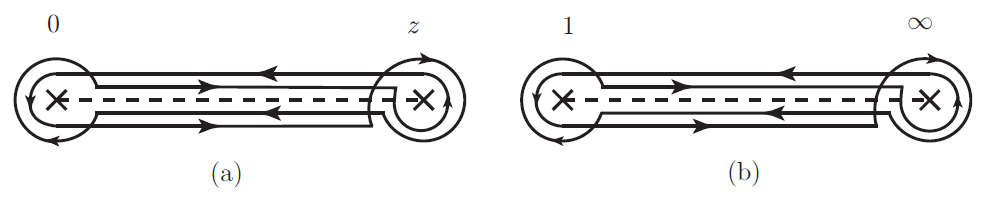
\includegraphics[width=0.6\linewidth]{fig/5.4.png}
	\caption{Pochhammer积分路径,(a)$S_a$,(b)$S_b$。}
\end{figure}

除了带些相位因子, $S_a$ 上的$ I_{S}(z) $就是$ [0,z] $上的积分, $S_b $上的就是 $[1,\infty)$ 上的积分:
\begin{align} &I_{S_{a}}(z)=\left(1-e^{2 \pi i a}\right)\left(1-e^{2 \pi i c}\right) I_{1}(z)\\ &I_{S_{b}}(z)= (1-e^{-2 \pi i(a+b+c)} )\left(1-e^{2 \pi i b}\right) I_{2}(z) \end{align}
其中
\begin{align} I_{1}(z) &=\int_{0}^{z} d v v^{a}(1-v)^{b}(z-v)^{c} \\ &=z^{1+a+b+c} \frac{\Gamma(a+1) \Gamma(c+1)}{\Gamma(a+c+2)} F(-b, a+1, a+c+2 ; z) \\ I_{2}(z) &=\int_{1}^{\infty} d v v^{a}(v-1)^{b}(v-z)^{c} \\ &=\frac{\Gamma(-a-b-c-1) \Gamma(b+1)}{\Gamma(-a-c)} F(-c,-a-b-c-1,-a-c ; z) \end{align}
都可写成超几何级数。借助超几何级数间的关系
\begin{equation}
	F(\alpha, \beta, \gamma ; z)=(1-z)^{\gamma-\alpha-\beta} F(\gamma-\alpha, \gamma-\beta, \gamma ; z) 
\end{equation}
可以看到,在 (5.44) 中取
\begin{equation}
	\alpha_{1}=2\left(\alpha_{0}-\beta_{n_{1}, m_{1}}\right), \quad \alpha_{2}=2\left(\alpha_{0}-\bar{\beta}_{n_{4}, m_{4}}\right), \quad \alpha_{3}=2\left(\alpha_{0}-\beta_{n_{3}, m_{3}}\right)
\end{equation}
得到的就是从$ \phi_{(1,2)} $零模条件推出的微分方程的解。

极小模型的自由场表示是相当有用的工具,可用来研究Virasoro代数的表示,例如构造零模向量,证明Kac的行列式猜想\footnote{M. Kato and S. Matsuda, Adv. Stud. Pure Math. 16 (1988) 205.}\footnote{A. Tsuchiya and Y. Kanie, Publ. RIMS 22 (1986) 259.}\footnote{G. Felder, Nucl. Phys. B 317 (1989) 215 [Erratum-ibid. B 324 (1989) 548].}。本书略过了这些主题,因为例如\footnote{山田泰彦,『共形場理論入門』,培風館, 2006.}\footnote{白石潤一,『量子可積分系入門』,SGC ライブラリ-28,サイエンス社,2003.}\footnote{鈴木淳史,『現代物理数学への招待—ランダムウォークからひろがる多彩な物理と数理』,SGC ライブラリ-47,サイエンス社,2006.}中已经解释得很详细了。
